\documentclass[11pt,french,a4paper]{report}
\usepackage[utf8]{inputenc}
\usepackage[left=2cm,right=2cm,top=2cm,bottom=2cm]{geometry}
\geometry{a4paper} 
\usepackage{graphicx} %Inclure images 
\usepackage{listings} %Style code C 
\usepackage[french]{babel} %Document en FR
\frenchbsetup{StandardLists=true}
\lstdefinestyle{customc}{ %Definition style code C
  belowcaptionskip=1\baselineskip,
  breaklines=true,
  frame=L,
  xleftmargin=\parindent,
  language=C,
  showstringspaces=false,
  basicstyle=\footnotesize\ttfamily,
}
\lstset{escapechar=@,style=customc}
\usepackage{pdflscape} %Vu Landscape
\usepackage{multicol} %Colonnes
\usepackage{enumitem}
\usepackage{pifont}
\usepackage{lastpage}
\usepackage{fancyhdr}
\pagestyle{fancy}
\usepackage{pdfpages}
\usepackage[pdftex]{graphicx}

%En tête / Pied de page
\fancyhead{}
\fancyfoot{}
\fancyhead[L]{
\includegraphics[scale=0.03]{../images/logo/logo_iutbeziers.png}}
\fancyhead[C]{Rapport de Stage - SuperBeeLive}
\fancyhead[R]{
\includegraphics[scale=0.3]{../images/logo/logoibmm.jpg}}
\fancyfoot[L]{\small Olivia SERENELLI-PESIN \normalsize}
\fancyfoot[R]{\thepage/\pageref{LastPage}}
\fancyfoot[C]{
\includegraphics[scale=0.03]{../images/logo/logo_abeille.png}}
\renewcommand{\footrulewidth}{0pt}
\renewcommand{\headrulewidth}{0,4pt}

%Indique qu'il faut appliquer le style sur tout le doc 
\makeatletter
\let\ps@plain=\ps@fancy
\makeatother

\begin{document}

%Page de garde
    \title{
        
\includegraphics[width=6cm]{../images/logo/logoibmm.jpg}\hspace{2cm} 
           
\includegraphics[width=6cm]{../images/logo/logo_lirmm_trans.png} \\
           \normalsize\textsc{}
           \hfill \\
           \hrulefill \\
           \hfill \\
           \LARGE \textbf{\uppercase{Rapport de Stage \\ Projet Superbeelive}} \\
           \hrulefill \\
           \hfill \\
           \Large{07 Avril 2019 - 05 Juillet 2019} \vspace*{5\baselineskip}
           }
         
    \author{
           \large{Stagiaire : \textbf{Olivia SERENELLI-PESIN}} \\
           \large{Tuteur : \textbf{Matthieu ROUSSET}} \\
            \bigskip \\
           \hfill \\
           \hfill \\
           \hfill \\
            
\includegraphics[width=4cm]{../images/logo/logo_iutbeziers.png}\hspace{7cm}
            
\includegraphics[width=5cm]{../images/logo/um_logo.png}
            \date{}
            }
\maketitle

\clearpage
\newpage 



\chapter*{Remerciements}

J’adresse mes remerciements aux personnes qui m’ont permis de réaliser ce stage dans l’équipe de SuperBeeLive. \\
Tout d’abord Matthieu Rouseet, initiateur du projet SuperBeeLive à l'IBMM (Institut Biomoléculaire Max Mousseron) 
qui m’a accueilli au sein de son équipe. \\

Ensuite, Capucine Carlier pour son accueil, pour ses nombreuses explications biologiques sur les abeilles ainsi que sa disponibilité 
afin de comprendre au mieux les enjeux et les besoins des biologistes pour mon projet. \\

Sébastien Druon pour m’avoir encadré, aidé à m’intégrer dans le milieu de la recherche et sur une multitude 
de sujets, aussi bien du point de vu universitaire que sur les tâches qui m’ont été confiées. \\

Enfin, toute l'équipe universitaire de l'IUT de Béziers qui m'aura appris sur beaucoup de sujets et rendu l'apprentissage
de différents domaines très intéressants. 

\begin{figure}[!h]
\centering
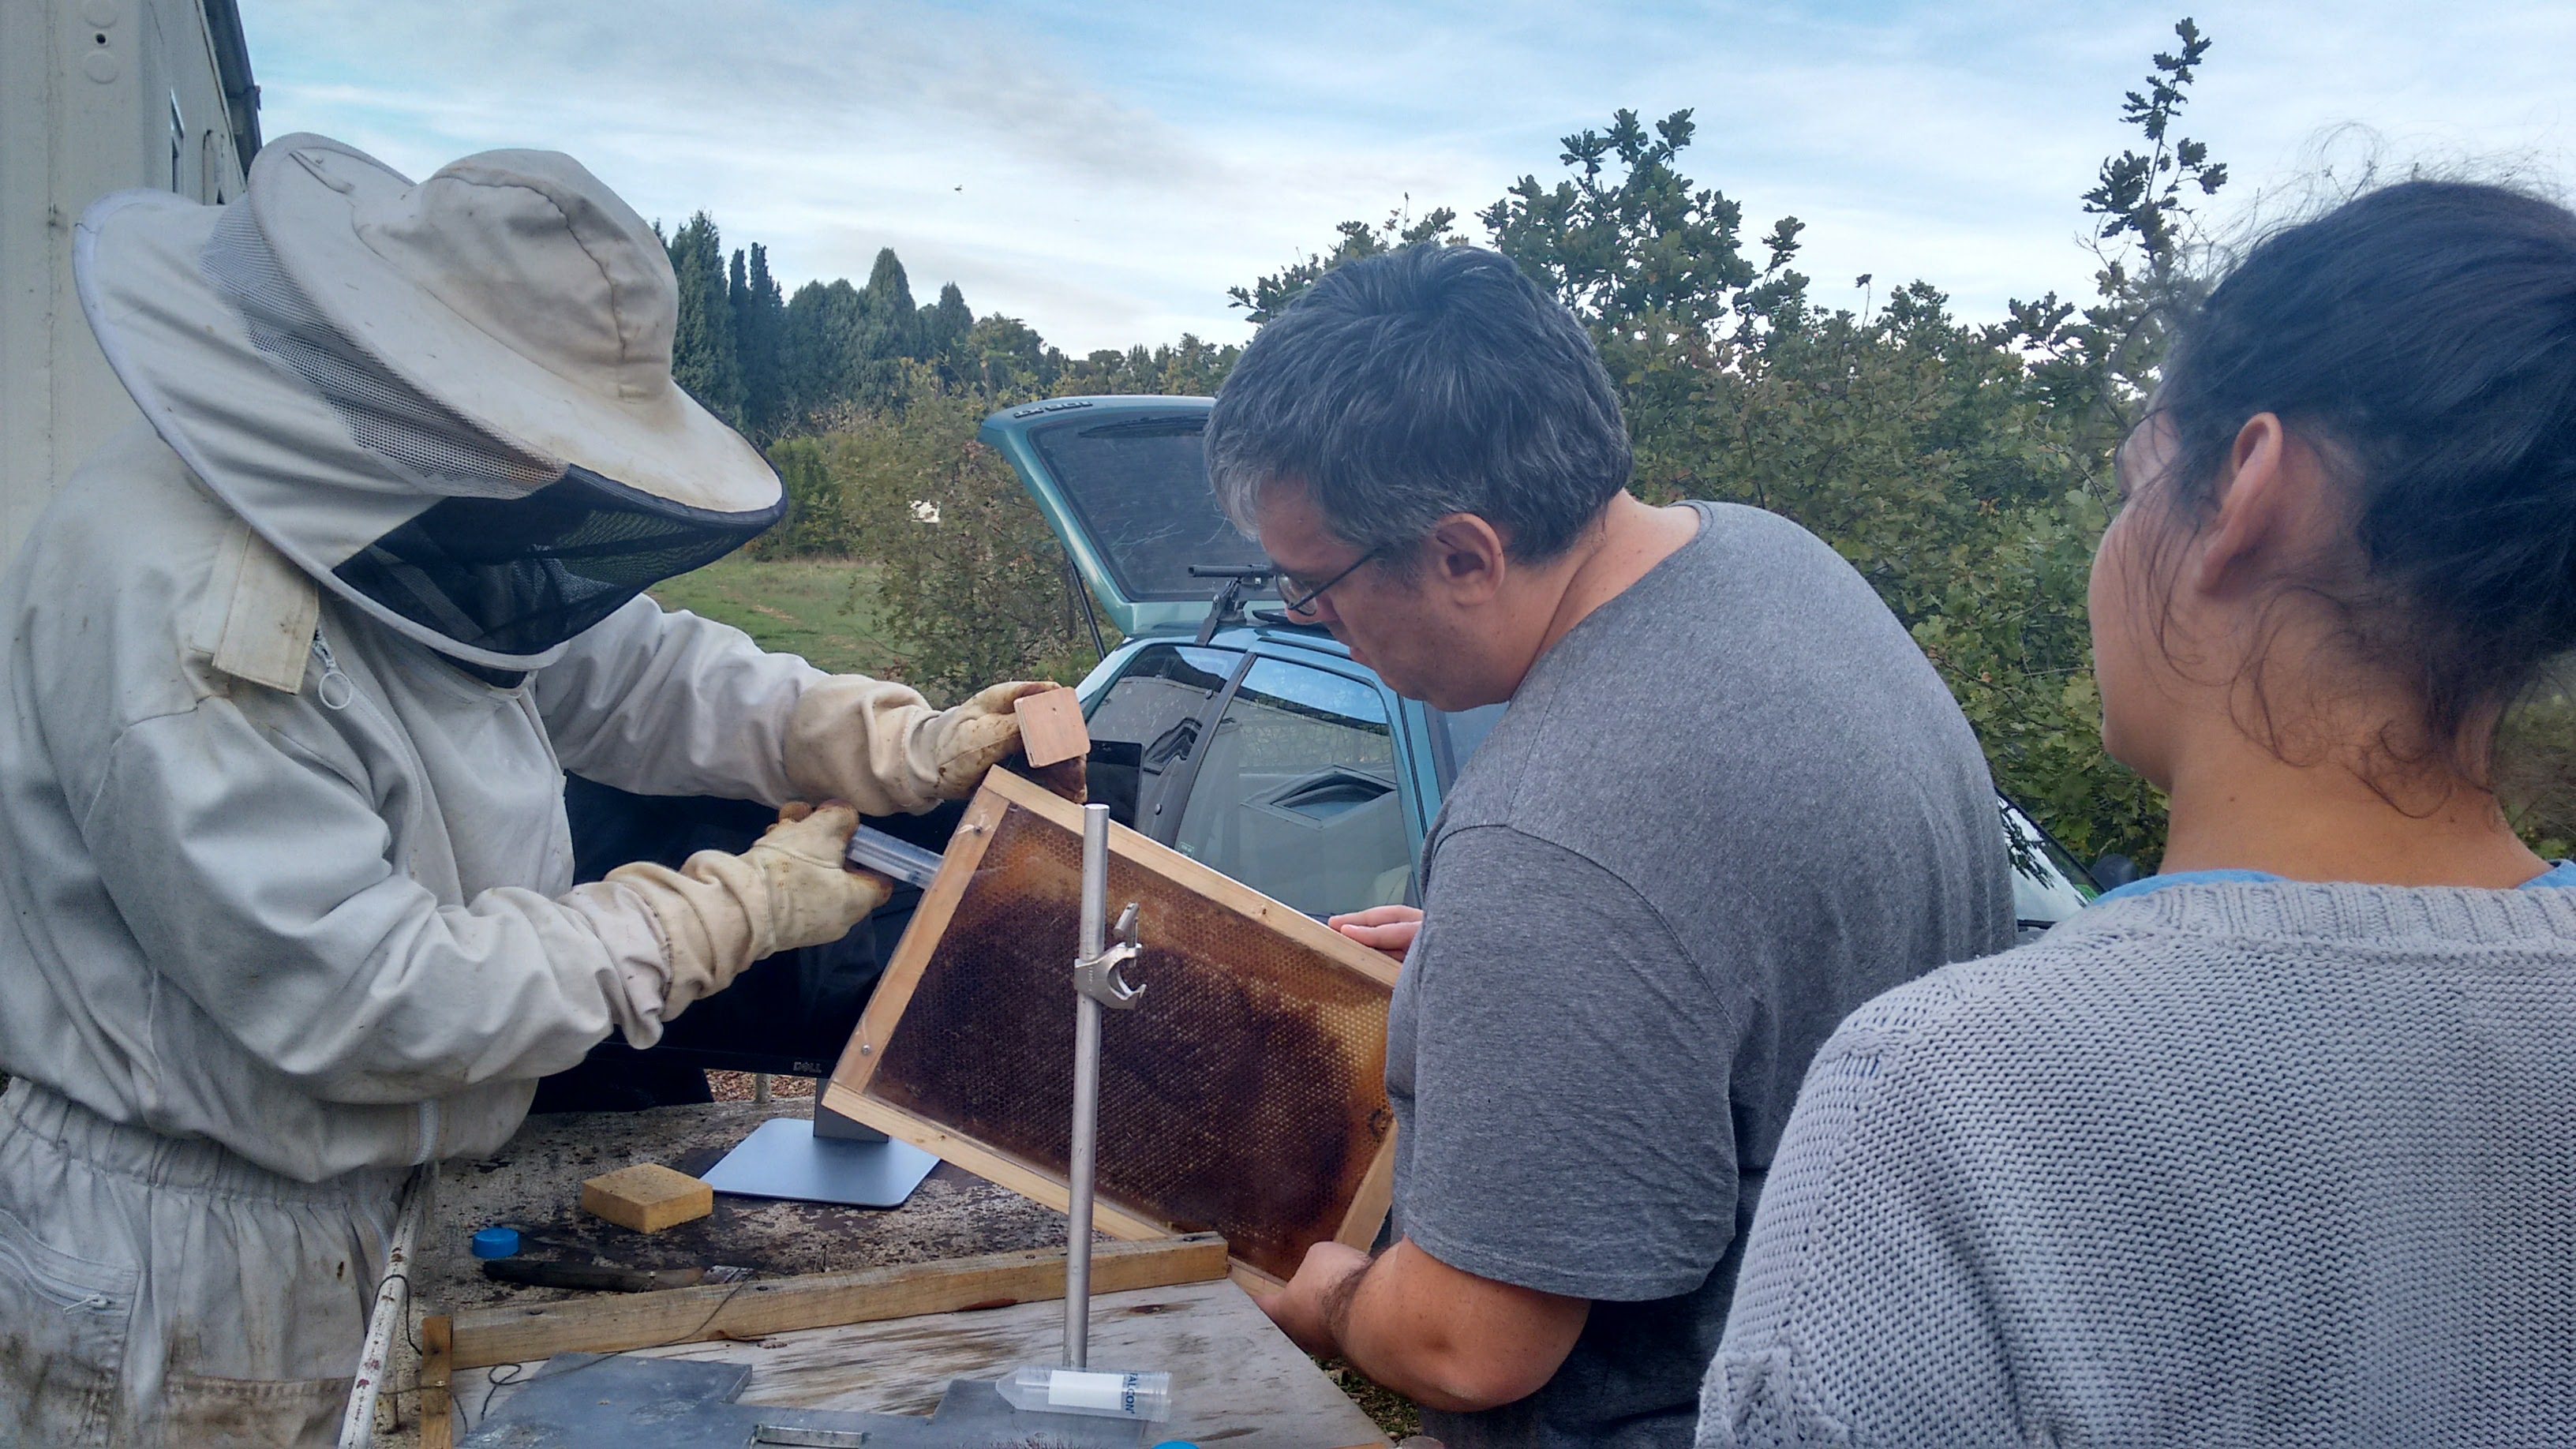
\includegraphics[width=10cm]{../images/photo/IMG_20171110_154804205_HDR.jpg}
\caption{Photo avec, de gauche à droite, Matthieu, Sébastien et Capucine au rucher.}
\label{ruche_pers}
\end{figure}

%TODO
%Typo pour %
%biblio logiciel


\tableofcontent

\clearpage

\chapter{Introduction : Présentation du projet de recherche}
\section{La structure d'accueil} 

Mon stage a été réalisé au sein d'un projet de recherche alliant biologie et technologie. 
Le projet étant réalisé par plusieurs laboratoires de recherches, j'ai dû évoluer aux seins de différentes organisations. 
Tout d'abord il y a mon employeur, l'Université de Montpellier, qui englobe d'autres structures où j'ai pu évoluer. 
L'université a été, pour moi, une entité administrative. \\ 
Avec elle, le CNRS (Centre National de Recherche Scientifique) accueille dans ses locaux le rucher expérimental \footnote{Voir figure \ref{ruches_ext}}
où l'équipe peut effectuer ses tests d'installation pour le projet. 
J'ai pu m'y rendre plusieurs fois afin d'observer les abeilles
et voir l'installation expérimentale au fur et à mesure. C'est également dans cette structure que nous aurons un serveur 
d'installé dans leur salle dédiée.\\
\begin{figure}[!h]
\centering
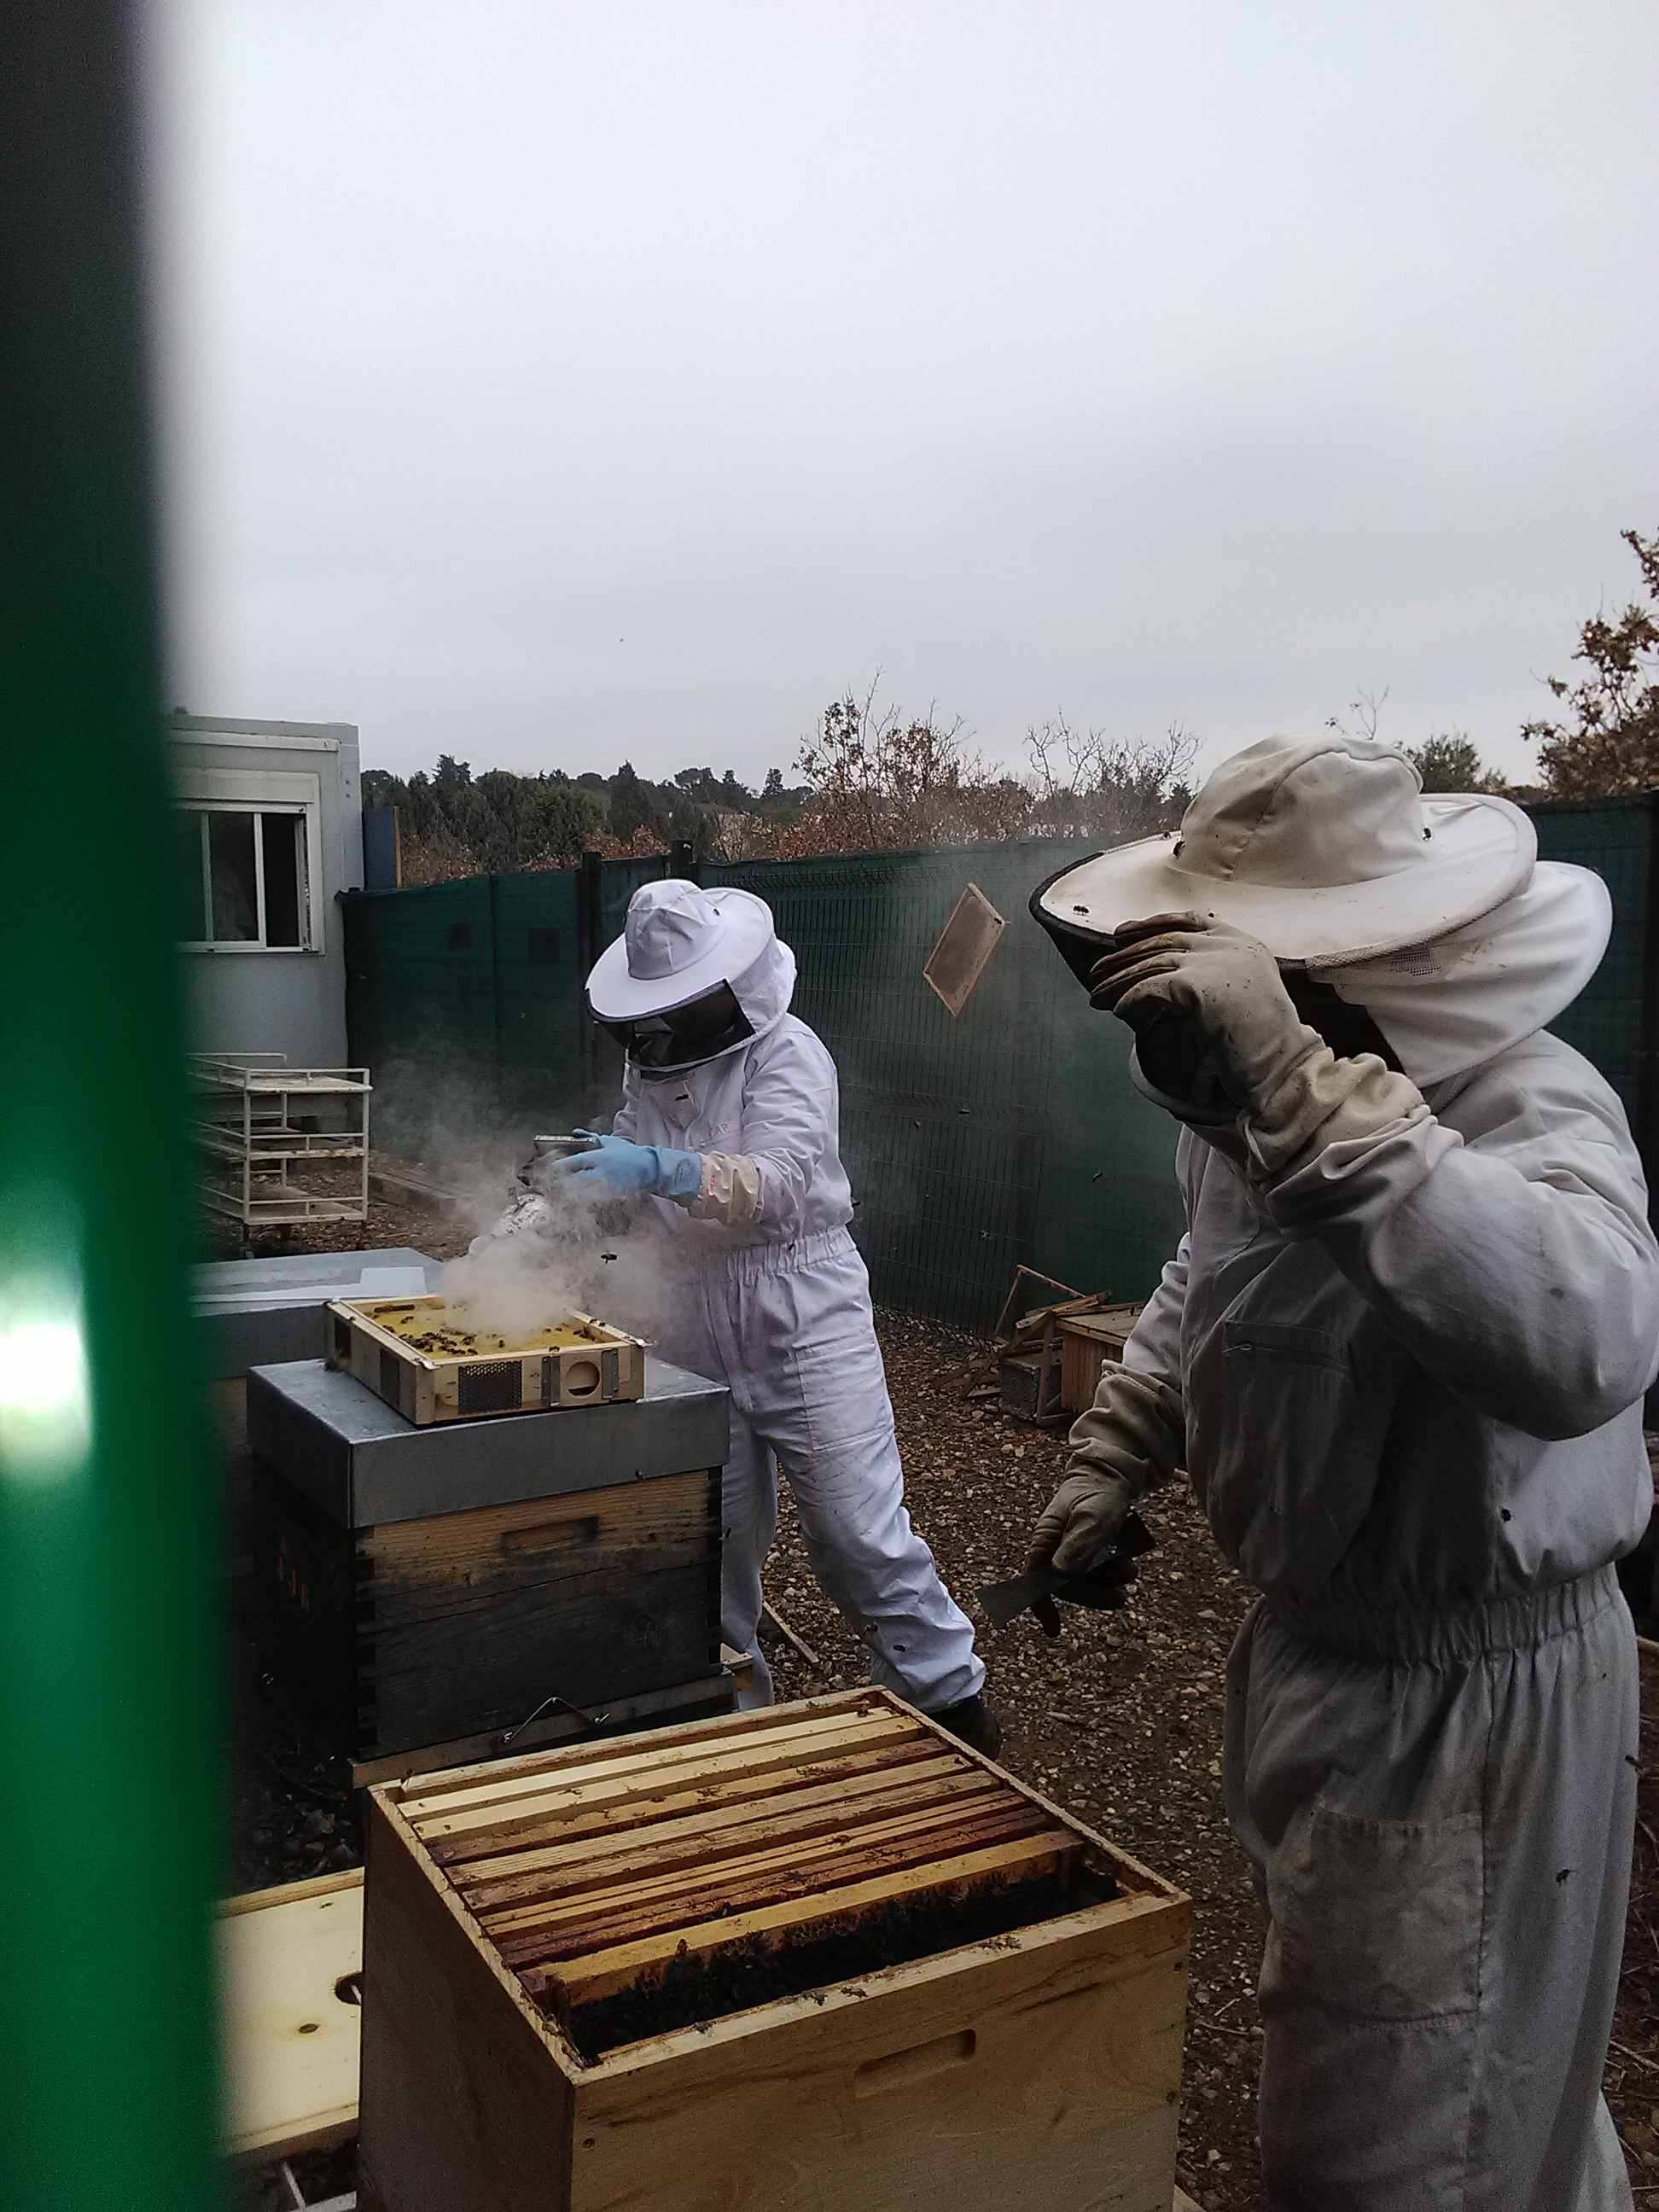
\includegraphics[width=10cm]{../images/photo/IMG_20180215_123536.jpg}
\caption{Photo de deux chercheurs sur les ruches extérieures du CNRS}
\label{ruches_ext}
\end{figure}
Ensuite, l'IBMM est le laboratoire qui a engagé l'argent lié au projet afin de pouvoir me recruter lors de ce stage. 
C'est également une structure qui a été seulement administrative de mon point de vu puisque j'ai été affectée dans 
les bureaux du LIRMM (Laboratoire d'Informatique, de Robotique et de Microélectronique de Montpellier), autre laboratoire de 
recherche, afin que je puisse être aux côtés de Sébastien Druon qui m'aura donné la grande majorité de mes tâches à effectuer. 
J'ai pu y avoir mon bureau en face du siens, me permettant d'être autonome, mais aussi de pouvoir faire
appel à lui facilement lorsque j'en avais besoin.\\

C'est dans ce contexte de recherche que j'ai pu découvrir et travailler sur le projet SuperBeeLive. \\ 


\section{Le projet SuperBeeLive}
 
La santé et le développement des abeilles sont aujourd’hui des questions de plus en plus étudiées. Les bouleversements
majeurs de notre planète et de l’activité humaine se traduisant par une augmentation alarmante de la mortalité
des colonies et une chute de la production du miel dans nos pays développés, il est urgent de se préoccuper de leur futur. 
La situation des abeilles domestiques alerte le pouvoir public sur l’accélération de la dégradation de la biodiversité des 
pollinisateurs domestiques et sauvages, et de la flore qui en dépend. Ces dégâts sont dûs, entre autres, à l’apparition 
et la prolifération d’espèces invasives pour les abeilles, provoquant maladies et détériorations. \\ 

Le projet consiste en la structuration de plusieurs collaborations existantes ou nouvelles autour du développement 
d’une ruche plate instrumentée destinée au monitorage détaillé de la santé de l’abeille et des écosystèmes. Son but est de
pouvoir répondre à des questions clé, notamment autour des mécanismes physiopathologiques et des maladies chroniques 
dûes aux parasites ainsi qu’aux altérations de l’écosystèmes et des qualités nutritives des produits des ruches. \\
Répondre à ces questions permettra de regrouper différentes solutions technologiques systèmatiques, 
automatiques et non-invasives à la collection de données usuelles déterminantes dans chacun des thèmes abordés.
Les différents travaux déjà effectués autour de ce sujet ne visaient qu’un seul type de problème à la fois, 
ne permettant pas une vision globale des difficultés rencontrées par les abeilles. Notre but est de réunir les différentes
données qui peuvent être utilisés pour étudier l’influence des éléments et événements extérieurs sur leur santé et leur cadre de vie.\\

Concrètement, l'équipe de SuperBeeLive va concevoir une ruche plate \footnote{Voir figures \ref{rpz_ruche} et \ref{photo_rucher}} afin d'y mettre 
en place plusieurs type  de capteurs (hygrométrie, vibrations, température interne et externe, etc) ainsi que des caméras qui filmeront 
l'intérieur et l'extérieur de la ruche. \\
En 2017, une affiche résumant le projet a été présentée lors du salon NUMEV (Solutions, Numériques, Matérielles, et 
Modélisation pour l'Environnement et le Vivant)\footnote{Voir Annexes, figure \ref{an1} }. \\ 

\begin{figure}[!h]
\centering
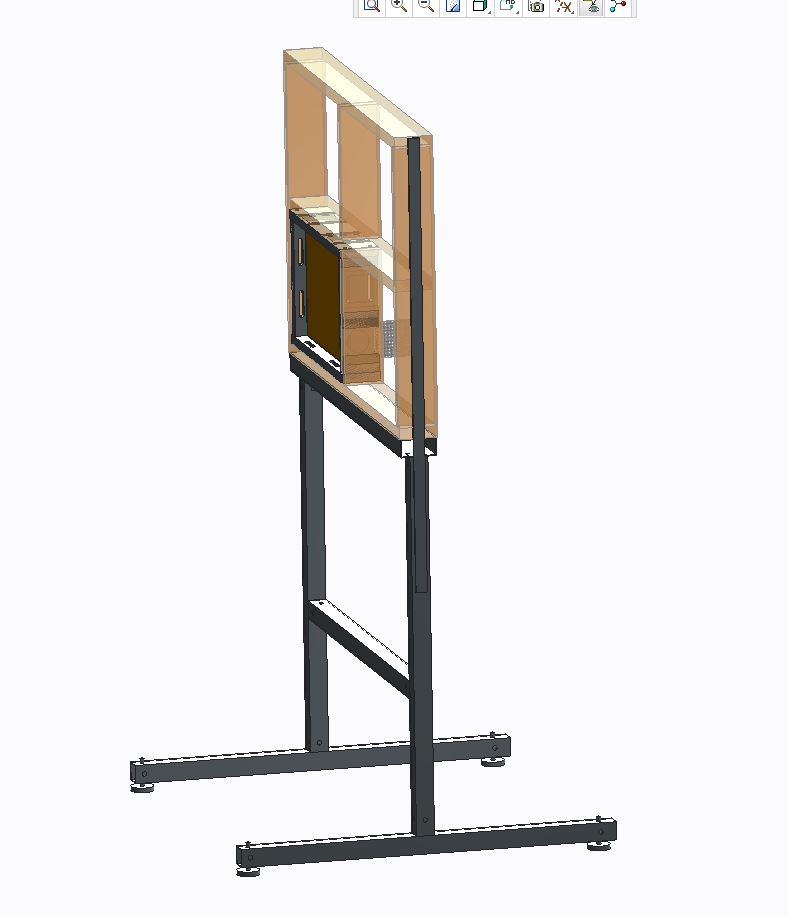
\includegraphics[scale=0.3]{../images/schema_ruche/supportrucheplate1.JPG}
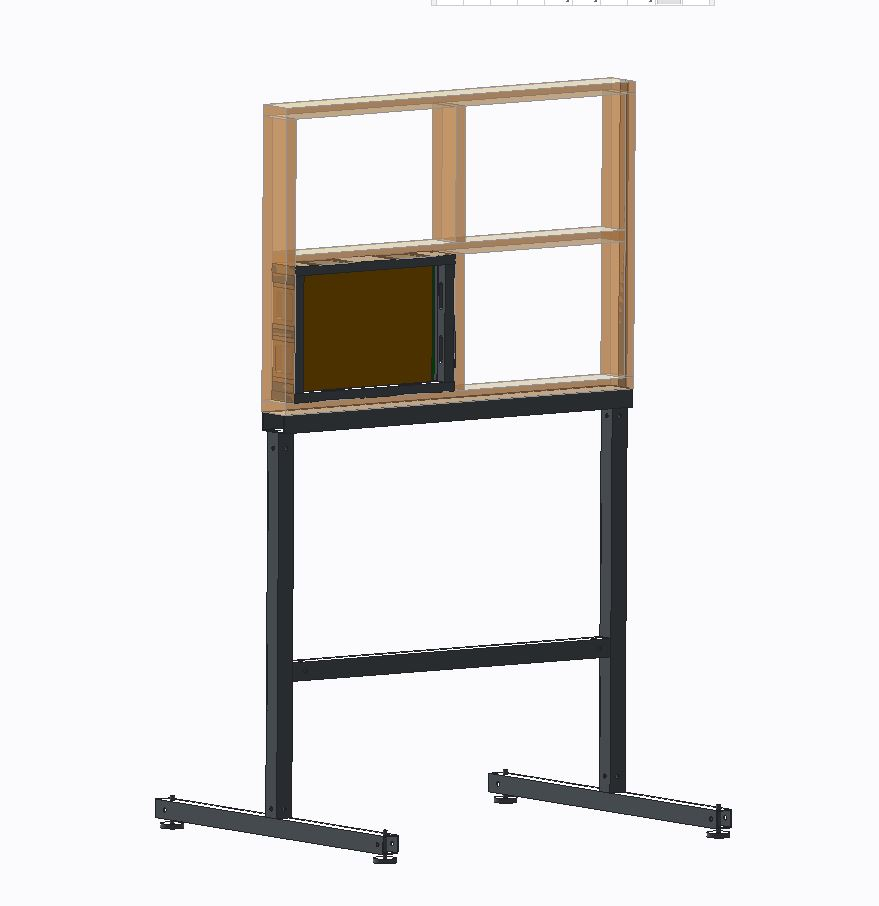
\includegraphics[scale=0.3]{../images/schema_ruche/supportrucheplate.JPG} 
\caption{Schéma 3D de la ruche plate}
\label{rpz_ruche}
\end{figure}

\begin{figure}[!h]
\centering
\includegraphics[scale=0.05,angle=270]{../images/photo/face_ruche.jpg}
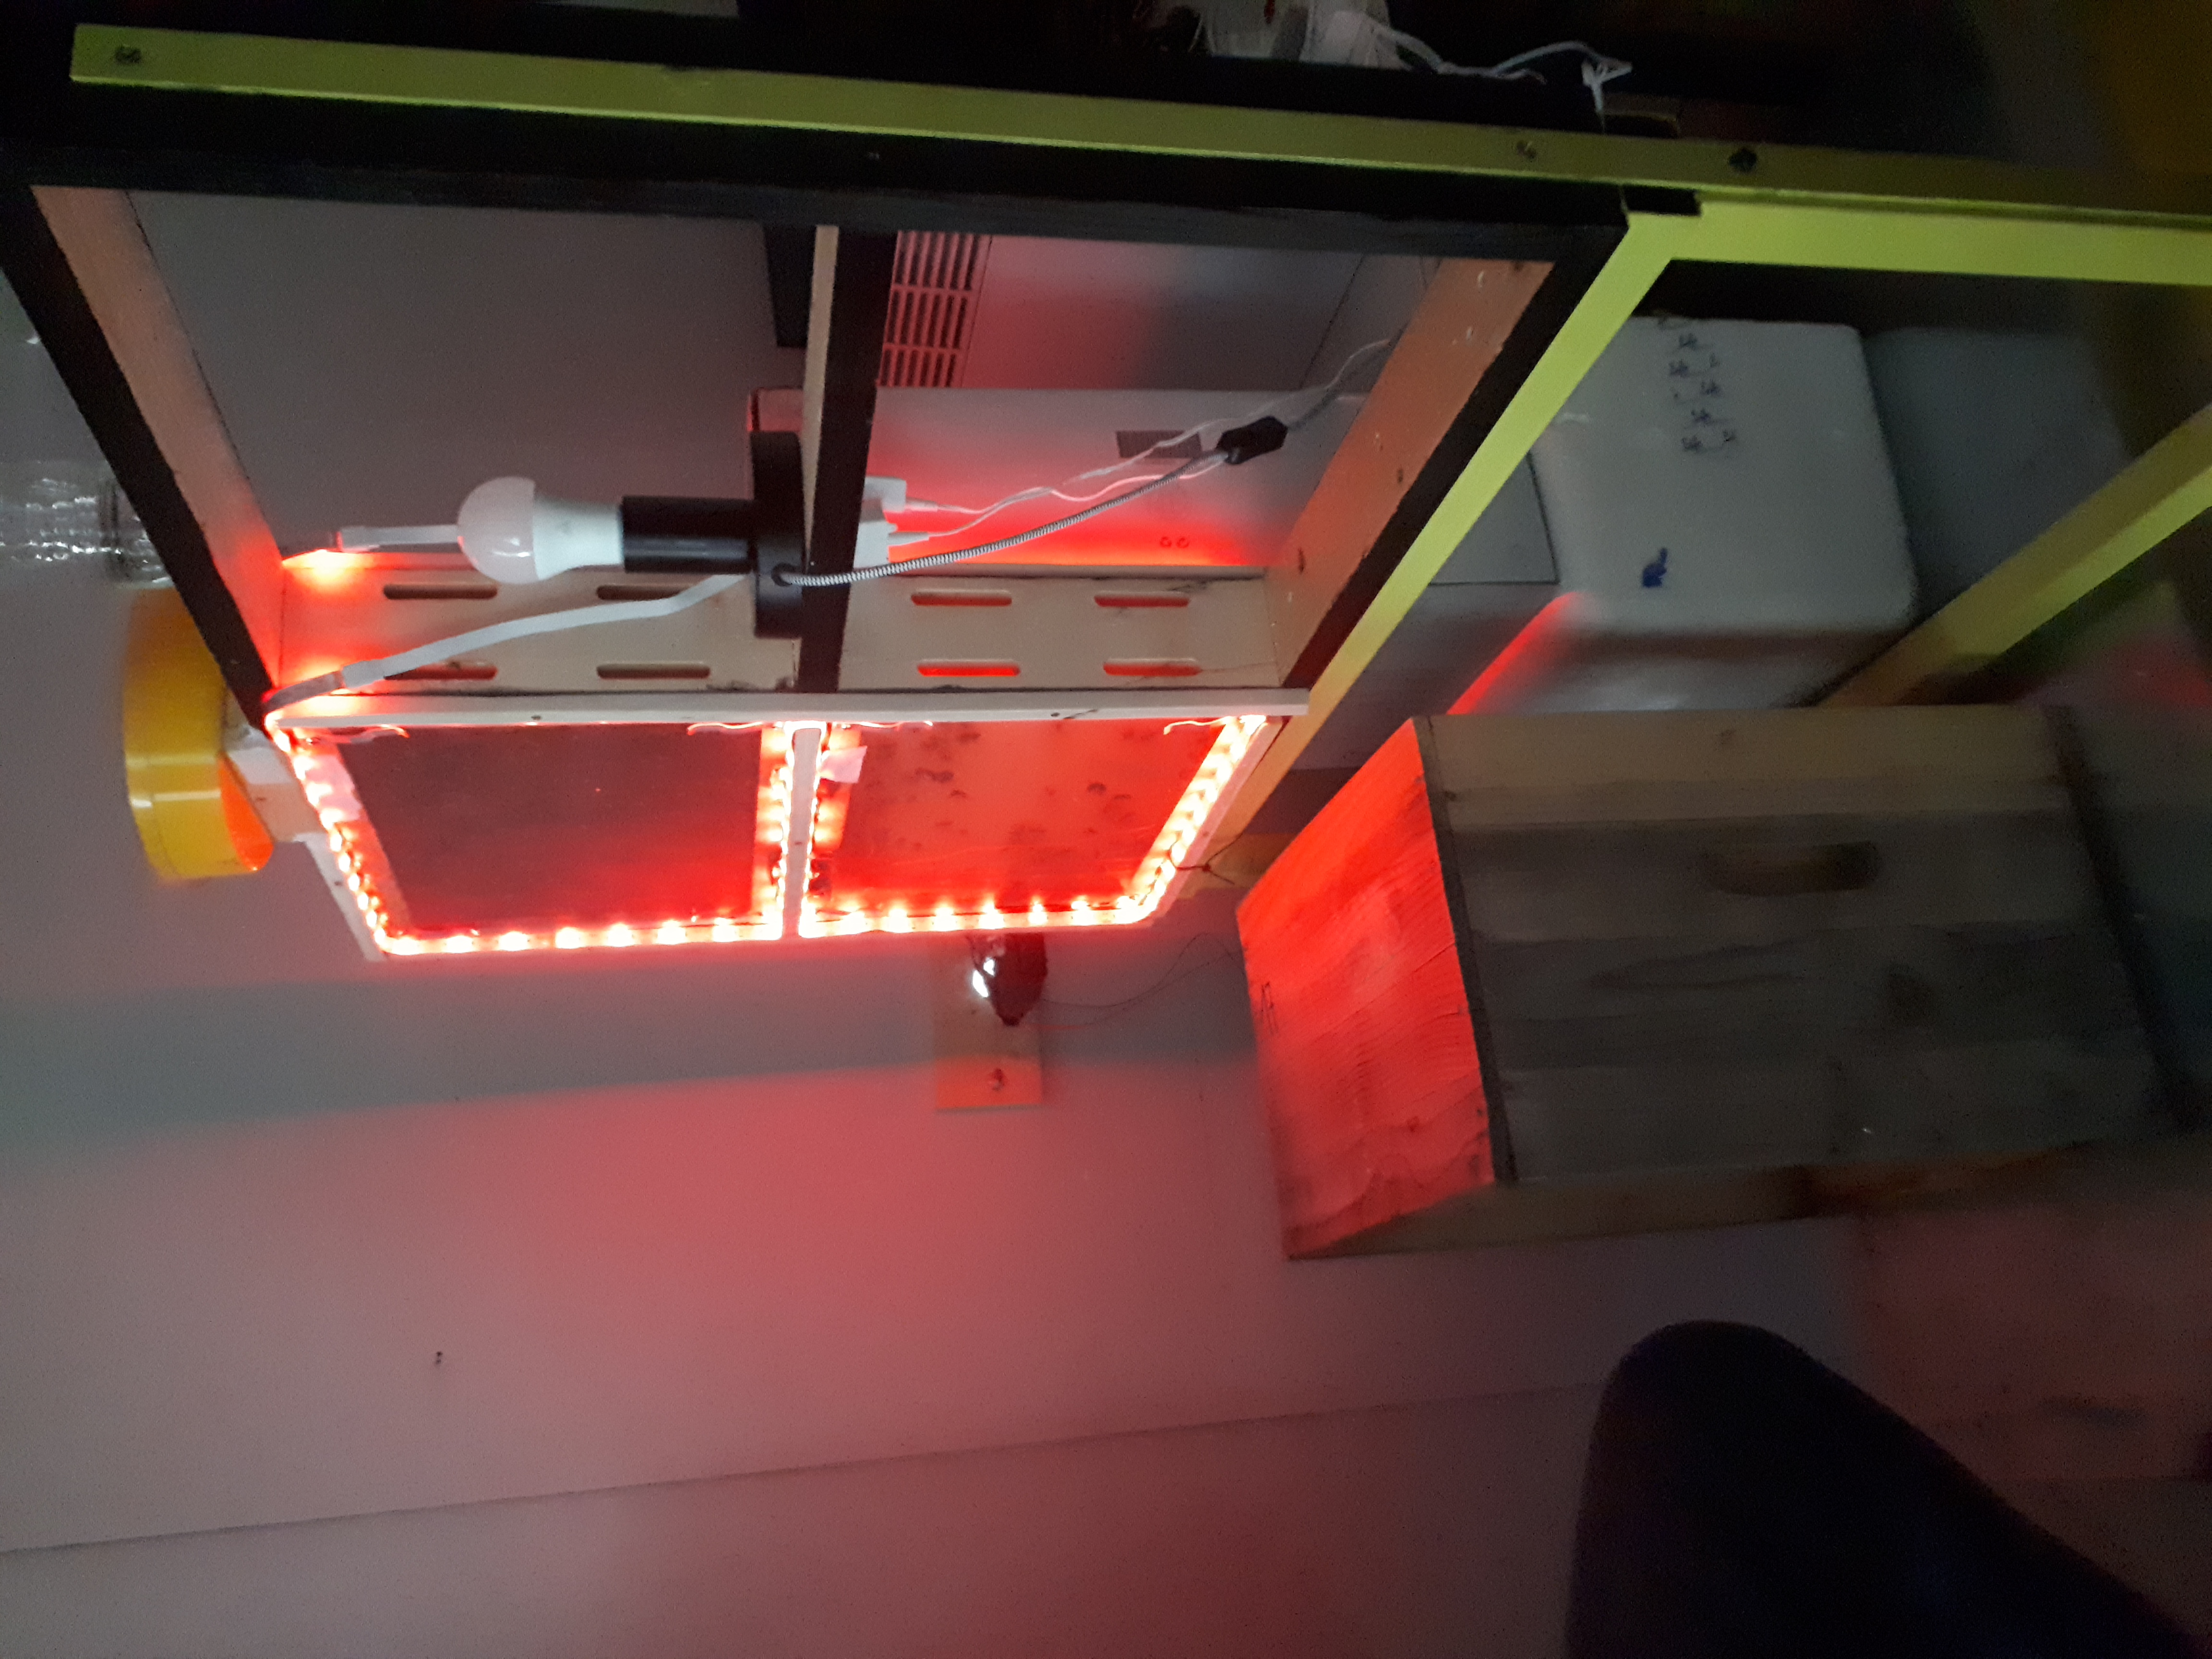
\includegraphics[scale=0.05,angle=270]{../images/photo/cote_ruche.jpg} \\
\caption{Photos de la ruche plate à mon arrivée}
\label{photo_rucher}
\end{figure}

Dans un premier temps, cette instrumentation nous permettra d'observer en temps réel la ruche et ses habitantes : 
les caméras nous donnerons une vision globale de ce qu'il s'y passe, aussi bien en intérieur pour observer leur 
comportement et tenter de repérer des parasites comme le varoa \footnote{Voir bibliographie \cite{ref11}}, 
qu'en extérieur pour y voir les dangers comme le frelon asiatique \footnote{Voir bibliographie \cite{ref12}}.
Couplée aux donnés récoltées à l'aide de la carte électronique et ses capteurs installés au centre de la ruche plate, 
nous pourrons avoir une vision complète et détaillée des événements et leur répercutions ponctuant la vie d'une colonie,
de sa naissance à sa mort. \\
Ces observations ont pour but d'être enregistrée, sauvegardées et commentées par les biologistes afin de construire une base
de donnée contenant plusieurs types de comportements reconnus comme le refroidissement de la ruche, les danses frétillante \footnote{Voir bibliographie \cite{ref10}}, 
etc.  
\\
Dans un second temps, cette base de donnée pourra être utilisée afin de créer des algorithmes repérant ces différents comportements
de manière automatisée. Cela nous permettrait, en plus d'avoir des données complètes, d'en avoir leur analyse en 
temps réel. Ces informations seront diffusées de deux façons. D'abord, elles seront partagées pour être étudiées par d'autres scientifiques, 
notamment les collaborateurs du projet SuperBeeLive. Le projet se veut aussi éducatif : une vitrine Web accessible au public 
sera créée présentant une ruche, ses données numériques et les vidéos commentées en direct par les algorithmes. \\


Ainsi, les ruches plates de SuperBeeLive permettront de fournir des données cruciales pour des futures recherches sur les 
abeilles. En plus, elles informeront le grand public sur leur importance et aux risques liées à nos activités humaines pour 
cette espèce et la biodiversité. 


\section{L'équipe}
L'équipe de recherche qui constitue le projet SuperBeeLive est répartie entre plusieurs laboratoires, je n'ai donc pas eu l'occasion
d'en rencontrer tous les acteurs, certains se trouvant même à l'étranger. Voici un schéma représentant globalement la structure
de l'équipe ainsi que les membres avec qui j'ai pu travailler \footnote{ Voir figure \ref{orga_sbl} }. \\

\begin{figure}[!h]
\centering
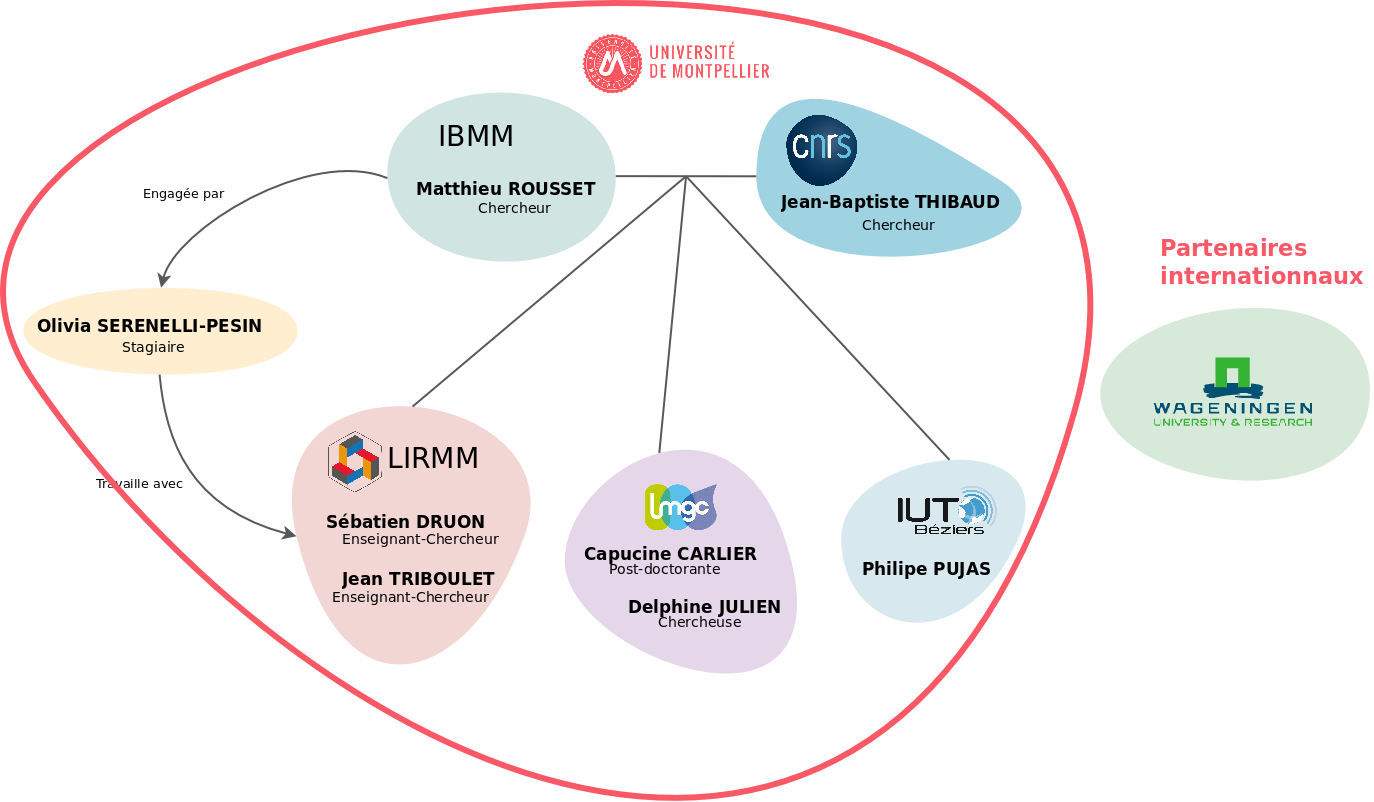
\includegraphics[scale=0.3]{../images/dia/organiramme_equipe_projet.png} \\
\caption{Organigramme de l'équipe SuperBeeLive}
\label{orga_sbl}
\end{figure}

Les laboratoires de recherche principaux sont l'IBMM (Institut Biomoléculaire Max Mousseron) 
et le CNRS (Centre National de la Recherche Française) sont représentés respectivement par Matthieu Rouseet et Jean-Baptsite Thibaud, 
tous deux chercheurs. \\
Les autres laboratoires actifs dans ce projet sont le LIRMM (Laboratoire d'Informatique, de Robotique, 
et de Microélectronique de Montpellier) et le LMGC (Laboratoire de Mécanique et Génie Civil). En plus de ces structures, 
des partenaires universitaires comme l'IUT de Béziers et l'Université de Wageningen, ouvrant à l'international,
permettent d'intégrer des étudiants. \\
Me concernant, j'ai été recrutée par l'IBMM et ai travaillé au LIRMM, travaillant principalement avec Mr Druon et 
Mr Triboulet. Les biologistes avec qui nous avons le plus été en contact lors de mon stage sont Matthieu Rouseet et Capucine Carlier. \\


\section{Mon rôle durant le stage}
Pour ce stage, plusieurs missions m'ont été affectées, une qui est devenue ma principale et d'autres, plus secondaires.\\

Comme dit plus haut, le but premier de l'installation des caméras sur la ruche est de pouvoir observer et récolter des informations
quant au comportement de la colonie, pour ensuite rendre cette détection automatique. Cette récolte d'information se fera par le 
biais d'annotations appliquées sur des enregistrements vidéo du live. Elles permettront de décrire ce qu'il se passe sur la vidéo, 
avec du texte et des figures simples (cercle, encadrement, etc.).
De plus, on veut pouvoir trier les vidéos en fonctions de ce qu'il s'y passe à l'aide de mots clé (tags). 
Si sur une vidéo il y a la reine et une danse frétillante, alors on l'indiquera avec les tags correspondants. \\

Seulement, ce travail d'annotation ne peut pas être fait avec des outils basiques, déjà disponibles au public comme Adobe Première Pro, 
Filmora ou Windows Movie Maker. Bien que très utilisés, ils possèdent bien plus de fonctionnalités que nécessaires et il aurait été long
de former toutes personnes devant faire ce travail d'annotation. De plus, on aurait eu des risques de pertes de données, celle-ci
ne pouvant être rapatriées automatiquement avec ces outils. Il vaut mieux prévoir un rassemblement du travail effectué sur 
un seul et même serveur. \\

Ainsi, nous avons entrepris de créer un logiciel d'annotation. Il permettra de regarder en direct les caméras et 
les données des capteurs et de sauvegarder des morceaux de vidéos afin de pouvoir dessiner simplement dessus 
(encercler, mettre une flèche, encadrer, etc) et écrire quelques mots sur ce qui y est observé.
Ces vidéos seraient sauvegardées dans un fichier contenant la vidéo et les annotations et pourront être 
visualisés de nouveau dans ledit logiciel, mais aussi dans un lecteur plus classique, sans les annotations. \\
Au final, l'application allégera le travail des biologistes, qui auront un outil sur-mesure pour annoter les vidéos, 
mais aussi celui de M. Druon et M. Triboulet, pour qui il sera plus simple de récupérer et travailler avec les données.\\

Il est évident que dans un tel projet, beaucoup de données seront transmises et stockées. Ainsi, toute une partie d'administration 
réseau est à installer et gérer. Dans notre cas, nous avons deux tâches importantes.\\
D'abord, la question du stockage des données commençait à se poser lors de mon arrivée en stage. Il fallait choisir, acheter, installer
puis configurer un serveur de stockage dans la salle serveur du CNRS.\\
Ensuite, le rucher du CNRS où notre ruche expérimentale est installée n'a pas de configuration réseau déjà établie. 
Une connexion par fibre optique est prévue, mais la suite de l'installation devra être gérée par nous-même. Comme pour le serveur, 
il faudra choisir, installer et configurer un switch dans le rucher.\\
Pour ces deux tâches, la même problématique est soulevée : il faudra penser au grand nombre de données qui devront transiter sur le 
réseau et donc prévoir du matériel adapté.\\

D'autres travaux auraient pu m'être affectées, comme le dimensionnement des caméras ou la construction des cartes électroniques
qui seront installées au centre de la ruche. Seulement, ces sujets s'éloignant de mon DUT Réseaux et Télécommunications et mes 
compétences et connaissances dans ces deux domaines étant limitées pour le moment, je n'ai pas eu à travailler dessus.\\
Cependant, la possibilité d'un apprentissage lors d'école d'ingénieurs en systèmes embarqués a été évoquée, ce qui correspondrait 
à ces tâches qui pourraient m'être confiées plus tard.


\chapter{Développement d'une application : Beeterface}
Développer une application/un logiciel n'est pas une tâche facile. Au-delà de la partie technique avec la programmation, 
beaucoup d'autres choses sont à prendre en compte. L'utilisation que l'on va faire de l'application et le public visé 
doivent être étudiés. Ce sont ces informations qui permettent de définir plus finement comment le logiciel va être 
construit. \\
N'ayant pas de connaissance théorique sur comment construire un logiciel ergonomique, je me suis placée en tant qu'utilisatrice
et ai regardé comment les logiciels que j'avais l'habitude d'utiliser étaient construits.
C'est avec ces questionnements simples que Beeterface a commencé à prendre forme sur papier : en commençant par analyser les besoins et 
les contraintes. Puis en me penchant sur la partie technique avec la découverte de GTK 3.0, et la manière de coder proprement en liant
la partie graphique à la partie fonctionnelle. Enfin, voir ce que le deuxième programmeur, M. Druon, a fait ainsi qu'une vision sur ce qu'il reste 
à faire permet de mettre en commun et faire le point sur comment les choses doivent évoluer.
 
 \section{Analyse du besoin et des fonctionnalités exigées}
Outre les différents capteurs installés sur la ruche (son, vibration, température, hygrométrie, etc.), 
les biologistes ont également exprimé le besoin de pouvoir capturer des comportements particuliers de la colonie. 
De là vient la nécessité de pouvoir gérer de nombreuses caméras sur la ruche prototype. 
On pourra distinguer trois localisations distinctes pour ces caméras \footnote{ Voir figure \ref{sch_cam} }, 
correspondant à trois types de traitement d'image différents. \\

\begin{figure}[!h]
\centering
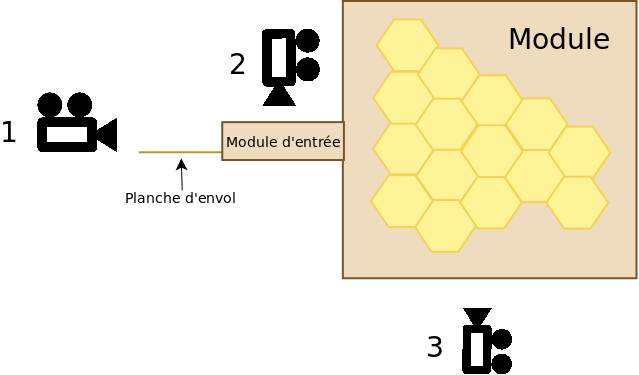
\includegraphics[scale=0.3]{../images/dia/schema_camera.png}
    \caption{Schéma représentant où vont se trouver les différentes caméras}
    \label{sch_cam}
\end{figure}
\begin{itemize}
  \item Les caméras situées sur la planche d'envol (1), tout d'abord, servent à surveiller 
  les alentours de la ruche. Elles permettent avant tout de
  mesurer le flux d'entrée/sortie des butineuses, mais également de détecter
  certains comportements, comme par exemple la ventilation forcée (une abeille
  bat des ailes afin de "pousser" de l'air frais vers l'intérieur de la ruche et faire
  diminuer la température). Ces caméras vont aussi servir à mesurer la
  "pression" des prédateurs sur le rucher, en mesurant le nombre de frelons
  asiatiques en embuscade (vol stationnaire) et le nombre d'abeilles
  capturées. Ces caméras sont au nombre de deux, formant une paire
  stéréoscopique afin de pouvoir effectuer des mesures 3D. \\
  En annexe, un lien vers une vidéo prise par l'équipe au début du projet est disponible. 
        On peut y voir une planche d'envol filmée et passée au ralenti \footnote{ Voir https://www.youtube.com/watch?v=jGhwq3n\_6mw&t=353s}. \\ 
 
  \item Les caméras situées sur le module d'entrée (2), quant à elles, servent à étudier
  les pelotes de pollen ramenées par les butineuses afin de reconnaître les
  plantes utilisées par les abeilles. Ces caméras sont caractérisées par de
  forts grossissements et sont associées à des éclairages pilotés par ordinateur
  (UV, IR) pour mesurer l'auto fluorescence des pollens.

  \item Enfin, les caméras montées sur chaque module (3) (1 par face du module) servent
  à détecter et surveiller les événements qui ont lieu sur le couvain et sur
  les alvéoles. Ces caméras doivent travailler dans des conditions de lumière
  particulières, car la reine et certaines castes d'abeilles sont sensibles à
  la lumière visible. Pour ne pas les perturber, le rucher est placé en
  lumière rouge ou infrarouge, ce qui correspond à des longueurs d'onde que les
  abeilles ne voient pas. Il est a noté que des caméras supplémentaires,
  purement infrarouges, seront également utilisées dans le cadre des travaux de
  l'IES, l'un de nos partenaires.
\end{itemize}

  Les flux d'images générés par ces caméras sont collectés sur un réseau privé,
  puis transférés à un serveur central. En fonction du besoin, ils pourront
  être enregistrés, renvoyés vers le site vitrine, renvoyés vers l'application d'annotation
  ou encore traités par les algorithmes qui sont mis au point par M. Triboulet et M. Druon. 
  Ces derniers se basent sur des réseaux de neurones artificiels afin de reconnaitre des comportements
  (danse, ventilation, etc) de façon automatique. \\

Au vu de la description générale de l'utilisation des vidéos ainsi qu'après une discussion avec l'équipe, le logiciel devrait 
pouvoir permettre de : \\
\begin{itemize}[itemsep=0cm,topsep=0cm]
    \item Visualiser les caméras en direct
    \item Démarrer la capture vidéo à tout moment 
    \item Ajouter un système de tag par mots clé afin de pouvoir trier facilement les vidéos 
    \item Avoir plusieurs types d'annotations (entourer, marquer, avoir des mouvements, etc.) 
    \item Retrouver toutes les mesures de la ruche (températures, horaires, numéro de caméra, de ruche, de cadre, etc.)  
    \item Connaître l'auteur d'une annotation 
    \item Pouvoir re visualiser les vidéos 
    \item Pouvoir re modifier les vidéos 
\end{itemize} \\
Afin de répondre à ces besoins, nous avons imaginé l'application "Beeterface" \footnote{Voir figure \ref{sch_beeterface}}.

\begin{landscape}
\begin{figure}[!h]
\begin{center}
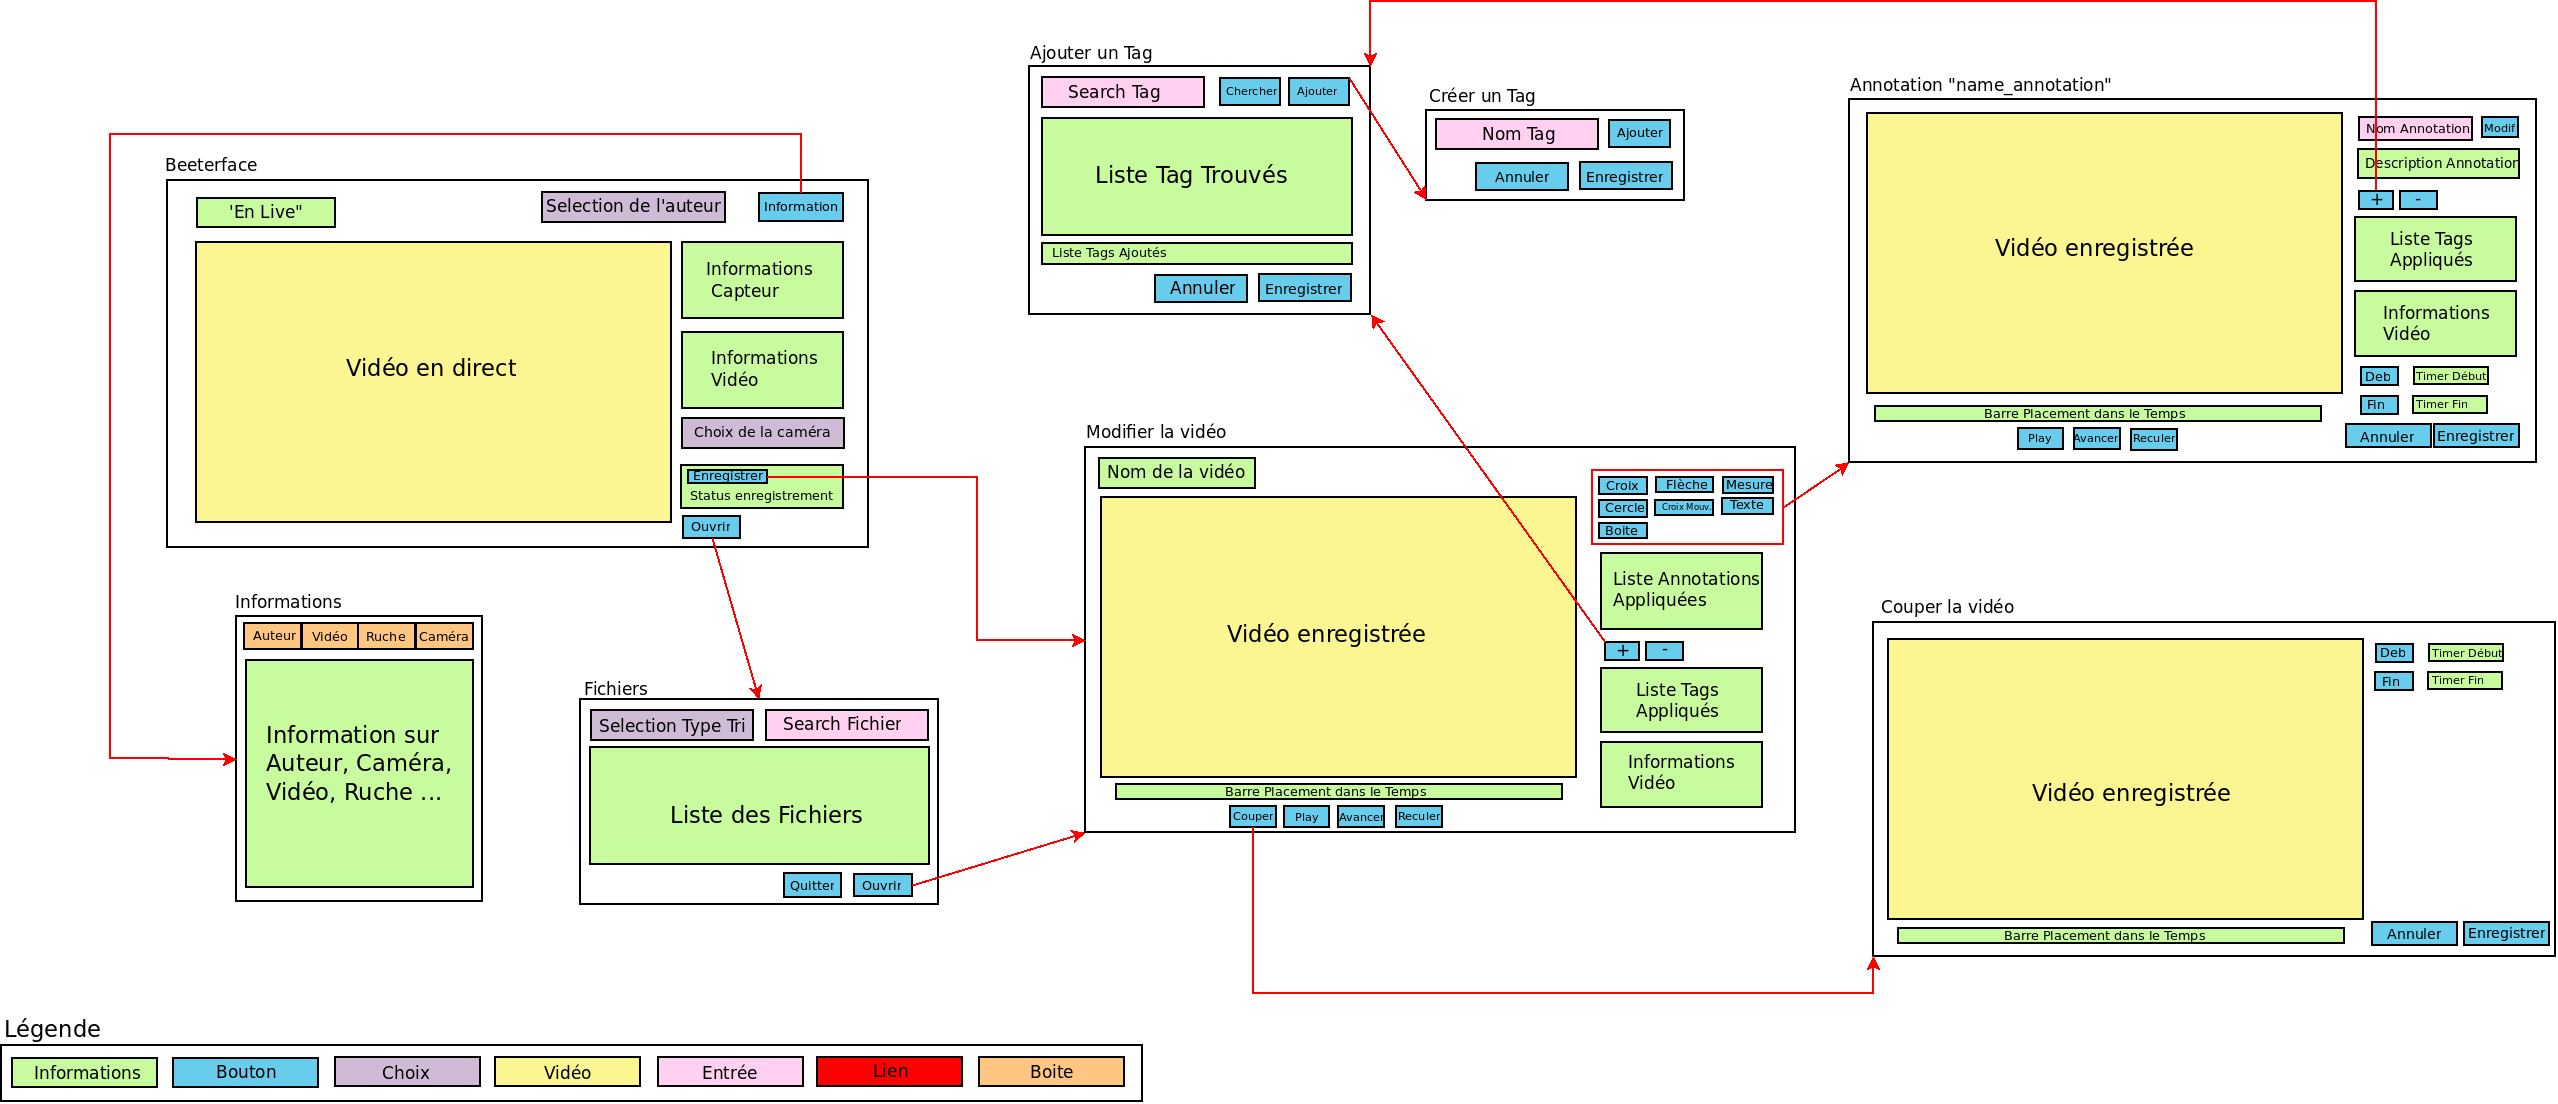
\includegraphics[scale=0.2]{../images/dia/schema_interface.png}
    \setlength{\columnseprule}{0,3}
\begin{multicols}{2}
    \begin{itemize}[label=\ding{241}, leftmargin=*,parsep=0cm,itemsep=0cm,topsep=0cm]
        \item Informations remontées : valeurs numériques ou textuelles. 
        \item Bouton : bouton cliquable.
        \item Choix : permet de choisir entre plusieurs valeurs prédéfinies.
        \item Vidéo : image fixe où sera placée la vidéo une fois cette partie codée.
        \item Entrée de texte : endroit où l'utilisateur peut écrire. 
        \item Boite : type de contenant particulier. 
        \item Lien : lien entre un bouton et une fenêtre. 
    \end{itemize}
\end{multicols}
    \caption{Schéma reprenant la structure de Beeterface}
    \label{sch_beeterface}
\end{center}
\end{figure}

\end{landscape}
            
\dotfill \\

\Large Fenêtre Principale - Beeterface \normalsize \\
    Première fenêtre ouverte. Permet de visualiser les caméras en direct, d'enregistrer
    des vidéos. \\
            \large \textbf{Informations} \normalsize
     \begin{itemize}[label=\ding{238}, leftmargin=*,parsep=0cm,itemsep=0cm,topsep=0cm]
        \item "En Live" : indique que la vidéo présentée est en live.
        \item "Informations Capteur" : remonte les informations en direct des capteurs (date, heure, température etc).
        \item "Informations de la Vidéo" : remonte les informations d'où est filmée la vidéo (ruche, caméra, numéro de cadre etc).
        \item "Statut enregistrement" : indique où en est l'enregistrement par rapport à la limite de temps maximale d'une vidéo à
               l'aide d'une barre se remplissant au fur et à mesure.
    \end{itemize}
            \large \textbf{Boutons} \normalsize
     \begin{itemize}[label=\ding{238}, leftmargin=*,parsep=0cm,itemsep=0cm,topsep=0cm]
        \item "Information" : Ouvre la fenêtre "Informations".
        \item "Enregistrer" : Permet de lancer l'enregistrement d'une vidéo. Pendant l'enregistrement, change de label et
        devient "Arrêter". Une fois l'enregistrement arrêté, ouvre la fenêtre "Modifier la vidéo".
        \item "Ouvrir" : Ouvre la fenêtre ""Fichiers".
    \end{itemize}
            \large \textbf{Choix} \normalsize
     \begin{itemize}[label=\ding{238}, leftmargin=*,parsep=0cm,itemsep=0cm,topsep=0cm]
        \item "Sélection de l'auteur" : permet de sélectionner l'auteur courant parmis une séléction (Capucine, Sébastien, Olivia, Matthieu, etc.).
        \item "Choix de la caméra" : permet de séléctionner la caméra à visualiser.
    \end{itemize}
            \large \textbf{Vidéo} \normalsize
     \begin{itemize}[label=\ding{238}, leftmargin=*,parsep=0cm,itemsep=0cm,topsep=0cm]
        \item "Vidéo en direct" = Direct de la caméra sélectionnée.
    \end{itemize}

\dotfill \\

\Large Fenêtre - Modifier la Vidéo\normalsize \\
    Fenêtre permettant de modifier une vidéo enregistrée ou de visualiser une vidéo déjà modifiée.
    C'est là que sont ajoutées les annotations. \\
\large \textbf{Informations}\normalsize
     \begin{itemize}[label=\ding{238}, leftmargin=*,parsep=0cm,itemsep=0cm,topsep=0cm]
        \item "Nom de la vidéo" : indique le nom de la vidéo, généré automatiquement.
        \item "Barre Placement dans le Temps" : barre de visualisation du temps de la vidéo, comme sur un player classique.
        \item "Liste Annotations Appliquées" : liste des annotations sur la vidéo. Permet de supprimer une annotation, de
        la cacher.
        \item "Liste Tags Appliqués" : liste des Tags appliqués sur la vidéo.
        \item "Informations Vidéos" : informations d'où a été filmée la vidéo au moment de l'enregistrement.
        \item 
\includegraphics[scale=0.05]{../images/logo/logo_ampoule} Ajouter "Information Capteurs" :
            avec les informations sur les capteurs au moment de l'enregistrement 
    \end{itemize}    
\large \textbf{Boutons}\normalsize
     \begin{itemize}[label=\ding{238}, leftmargin=*,parsep=0cm,itemsep=0cm,topsep=0cm]
        \item "Couper" : ouvre la fenêtre "Couper la vidéo".
        \item "Play" : lance la Vidéo. Le label se change en "stop" pour mettre en pause.
        \item "Avancer" : avance la vidéo de 5 secondes.
        \item "Reculer" : recule la vidéo de 5 secondes.
        \item "Croix", "Flèche", "Mesure", "Cercle", "Crois Mouv", "Texte", "Boite", "Croix Mouv.", "Texte", "Boite" : ouvrent
        leur fenêtre "Annotation "name\_annotation"" respective.
        \item "+" : ouvre la fenêtre "Ajouter un Tag"
        \item "-" : supprime un tag à sélectionner dans la liste.
    \end{itemize}
\large \textbf{Vidéo}\normalsize
    \begin{itemize}[label=\ding{238}, leftmargin=*,parsep=0cm,itemsep=0cm,topsep=0cm]
        \item "Vidéo enregistrée" : visualisation de la vidéo à modifier avec les annotations dessus.
    \end{itemize}

\dotfill \\
\clearpage

\Large Fenêtre - Annotation "name\_anotation"\normalsize \\
    Fenêtre qui permet de placer une nouvelle annotation. Elle change à quelques endroits en fonction
    du bouton utilisé pour appeler la fenêtre. \\
\large \textbf{Informations}\normalsize
    \begin{itemize}[label=\ding{238}, leftmargin=*,parsep=0cm,itemsep=0cm,topsep=0cm]
        \item "Barre Placement dans le Temps" : barre de visualisation du temps de la vidéo, comme sur un player classique.
        \item "Description Annotation" : description de l'annotation : comment l'utiliser, à quoi elle sert, à quoi elle ressemble.
        \item "Liste Tags Appliqués" : liste des Tags appliqués sur la vidéo.
        \item "Informations Vidéos" : informations d'où a été filmée la vidéo au moment de l'enregistrement.
        \item 
\includegraphics[scale=0.05]{../images/logo/logo_ampoule} Ajouter "Information Capteurs" :
            avec les informations sur les capteurs au moment de l'enregistrement. 
        \item "Timer Début" : indication du moment de la vidéo où l'annotation va débuter.
        \item "Timer Fin" : indication du moment de la vidéo où l'annotation va finir.
    \end{itemize}
\large \textbf{Boutons}\normalsize
    \begin{itemize}[label=\ding{238}, leftmargin=*,parsep=0cm,itemsep=0cm,topsep=0cm]
        \item "Play" : lance la Vidéo. Le label se change en "stop" pour mettre en pause.
        \item "Avancer" : avance la vidéo de 5 secondes.
        \item "Reculer" : recule la vidéo de 5 secondes.
        \item "Modif" : bouton avec une image de crayon. Quand on appuie dessus, l'image change en "OK" et l'entrée "nom annotation" devient éditable
        pour y entrer un nom reconnaissable par l'utilisateur. Quand on appuie de nouveau dessus, l'image redevient comme avant et
        l'information est sauvegardée et l'entrée "nom annotation" redevient non éditable.
        \item "+" : ouvre la fenêtre "Ajouter un Tag"
        \item "-" : supprime un tag à sélectionner dans la liste.
        \item "Deb" : fixe la valeur de "Timer Début" avec la valeur actuelle du timer de la vidéo.
        \item "Fin" : fixe la valeur de "Timer Fin" avec la valeur actuelle du timer de la vidéo.
        \item "Annuler" : ferme la fenêtre sans enregistrer les modifications.
        \item "Enregistrer" : ferme la fenêtre en enregistrant les modifications.
    \end{itemize}
\large \textbf{Entrée}\normalsize
    \begin{itemize}[label=\ding{238}, leftmargin=*,parsep=0cm,itemsep=0cm,topsep=0cm]
        \item "Nom Annotation" : permet de saisir le nom de l'annotation que l'utilisateur veut lui donner pour le reconnaître.
        De base pas modifiable. Fonctionne avec le bouton "Modif".
\large \textbf{Vidéo}\normalsize :
        \item "Vidéo enregistrée" : visualisation de la vidéo où mettre l'annotation.
    \end{itemize}

\dotfill \\
\Large Fenêtre - Informations \\ \normalsize 
    Fenêtre contenant des informations sur les différentes structures et leur éléments. Permet de retrouver les différentes ruches
    et leurs spécificités, les auteurs, les infos contenues dans "vidéo", "caméra" etc. Ne permet pas de modification. \\
\large \textbf{Information} \normalsize
    \begin{itemize}[label=\ding{238}, leftmargin=*,parsep=0cm,itemsep=0cm,topsep=0cm]
        \item "Information sur Auteur, Caméra, Vidéo, Ruche..." : affiche les informations correspondant à l'onglet sur lequel on se trouve.
    \end{itemize}
\large \textbf{Box} \normalsize
    \begin{itemize}[label=\ding{238}, leftmargin=*,parsep=0cm,itemsep=0cm,topsep=0cm]
        \item "Auteur", "Vidéo", "Ruche", "Caméra", etc : onglets permettant de sélectionner quel type d'information on veut visualiser.
    \end{itemize}
    
\includegraphics[scale=0.05]{../images/logo/logo_ampoule} Ajouter une entrée permettant une recherche rapide ? \\

\dotfill \\

\Large Fenêtre - Couper la vidéo\normalsize \\
    Fenêtre permettant de redécouper la vidéo. \\
\large \textbf{Informations}\normalsize
    \begin{itemize}[label=\ding{238}, leftmargin=*,parsep=0cm,itemsep=0cm,topsep=0cm]
        \item "Barre Placement dans le Temps" : barre de visualisation du temps de la vidéo, comme sur un player classique.
        \item "Timer Début" : indication du moment de la vidéo où l'annotation va débuter.
        \item "Timer Fin" : indication du moment de la vidéo où l'annotation va finir.
    \end{itemize}
\large \textbf{Boutons}\normalsize
    \begin{itemize}[label=\ding{238}, leftmargin=*,parsep=0cm,itemsep=0cm,topsep=0cm]
        \item "Deb" : fixe la valeur de "Timer Début" avec la valeur actuelle du timer de la vidéo.
        \item "Fin" : fixe la valeur de "Timer Fin" avec la valeur actuelle du timer de la vidéo.
        \item "Annuler" : ferme la fenêtre sans enregistrer les modifications.
        \item "Enregistrer" : ferme la fenêtre en enregistrant les modifications.
    \end{itemize}
\large \textbf{Vidéo}\normalsize
    \begin{itemize}[label=\ding{238}, leftmargin=*,parsep=0cm,itemsep=0cm,topsep=0cm]
        \item "Vidéo enregistrée" : visualisation de la vidéo à découper.
    \end{itemize}

\dotfill \\

\Large Fenêtre - Ajouter un tag\normalsize \\
    Fenêtre permettant de visualiser les tags disponnibles pour en sélectionner une liste à ajouter sur la vidéo
    ou sur une annotation. \\
\large \textbf{Informations}\normalsize
    \begin{itemize}[label=\ding{238}, leftmargin=*,parsep=0cm,itemsep=0cm,topsep=0cm]
        \item "Liste Tag Trouvés" : listes des tags trouvés en fonctions des critères de recherche.
        Affiche tous les tags disponnibles par ordre alphabétique si pas de recherche faite .
        \item "Liste Tags Ajoutés" : listes les tags sélectionnés pour être ajoutés à la vidéo ou l'annotation.
    \end{itemize}
\large \textbf{Boutons} \normalsize
    \begin{itemize}[label=\ding{238}, leftmargin=*,parsep=0cm,itemsep=0cm,topsep=0cm]
        \item "Chercher" : lance la recherche de tag en fonction de ce qui est écrit dans "Search Tag"
        \item "Ajouter" : ouvre la fenêtre  "Créer un Tag"
        \item "Annuler" :  ferme la fenêtre sans enregistrer les modifications.
        \item "Enregistrer" : ferme la fenêtre en enregistrant les modifications.
    \end{itemize}
\large \textbf{Entrée}\normalsize
    \begin{itemize}[label=\ding{238}, leftmargin=*,parsep=0cm,itemsep=0cm,topsep=0cm]
        \item "Search Tag" : entrée de recherche où on peut entrer un mot clé à chercher pour trouver un tag correspondant.
    \end{itemize}
    
\includegraphics[scale=0.05]{../images/logo/logo_ampoule} Ajouter la possibilitée de voir les tags ajoutés 
            les plus récent ? \\ 

\dotfill \\

\Large Fenêtre - Créer un Tag\normalsize \\
    Fenêtre permettant de créer un nouveau tag dans le dictionnaire si il n'en existe pas déjà
    un correspondant à ce que l'utilisateur veut. \\
\large \textbf{Boutons}\normalsize
    \begin{itemize}[label=\ding{238}, leftmargin=*,parsep=0cm,itemsep=0cm,topsep=0cm]
        \item "Ajouter" : ajoute comme nouveau tag ce qui est entrée dans "Nom Tag"
        \item "Annuler" : ferme la fenêtre sans enregistrer les modifications.
        \item "Enregistrer" : ferme la fenêtre en enregistrant les modifications.
    \end{itemize}
\large \textbf{Entrée}\normalsize
    \begin{itemize}[label=\ding{238}, leftmargin=*,parsep=0cm,itemsep=0cm,topsep=0cm]
        \item "Nom Tag" : entrée où l'utilisateur doit indiquer le nom du nouveau tag qu'il désire.
    \end{itemize}
    
\includegraphics[scale=0.05]{../images/logo/logo_ampoule} Ajouter la possibilitée de voir les tags ajoutés 
            les plus récent ? \\ 
    
\includegraphics[scale=0.05]{../images/logo/logo_ampoule} Ajouter une vérification des tags qui pourraient 
    ressembler au nouveau que l'utilisateur veut ajouter pour éviter les doublons ? \\

\dotfill \\

\Large Fenêtre - Fichier\normalsize \\
    Fenêtre permettant de voir les fichiers vidéo existant et de les trier suivant différents critères. \\
\large \textbf{Informations}\normalsize 
    \begin{itemize}[label=\ding{238}, leftmargin=*,parsep=0cm,itemsep=0cm,topsep=0cm]
        \item "Liste des Fichiers" : liste des fichiers en fonction du critère de tri choisit. Si pas de critère sélectionné,
        c'est rangé par ordre alphabétique.
    \end{itemize}
\large \textbf{Boutons}\normalsize
    \begin{itemize}[label=\ding{238}, leftmargin=*,parsep=0cm,itemsep=0cm,topsep=0cm]
        \item "Quitter" : quitte l'explorateur de fichier sans rien ouvrir.
        \item "Ouvrir" : ferme l'explorateur de ficher en ouvrant le fichier séléctionné dans la liste de "Liste des Fichiers dans une
        fenêtre "Modifier la vidéo"
    \end{itemize}
\large \textbf{Choix}\normalsize
    \begin{itemize}[label=\ding{238}, leftmargin=*,parsep=0cm,itemsep=0cm,topsep=0cm]
        \item "Selection Type Tri" : permet de choisir par quel critère trier les vidéos : par caméra, auteur, date, ruche, lieu, tag etc
    \end{itemize}
\large \textbf{Entrée}\normalsize
    \begin{itemize}[label=\ding{238}, leftmargin=*,parsep=0cm,itemsep=0cm,topsep=0cm]
        \item "Search Fichier" : permet d'entrer un mot-clé pour affiner la recherche. Se couple à la recherche en fonction du type de tri
        choisi.
    \end{itemize}
\dotfill \\
Bien sûr, celle-ci a connu beaucoup d'évolutions au cours de son développement : au fur et à mesure de l'avancement,
nous nous rendions compte de certaines éventualités que nous n'avions pas imaginé et que nous avons intégré à la volée. 
Ainsi, ce schéma correspond à l'application actuelle mais n'avait pas été vu comme tel au début. 

    \section{Contraintes} 
Le langage de départ pour coder l'interface et ses fonctionnalités, que nous pourrons familièrement nommer partie moteur 
et partie graphique, m'a été imposé. \\
C'est donc en C \footnote{Voir bibliographies \cite{ref5} \cite{ref8}} que j'ai dû réfléchir à la façon de préparer et lier ces deux parties. Ce langage a été choisi tout simplement 
parceque c'est  le langage que M. Druon a pour habitude d'utiliser pour ce type de projet. \\
La partie "moteur" peut être développée en C sans trop d'ajouts de librairies annexes autres que celles dites basiques 
(stdlib, stdio). 
Cependant, nous avons dû utiliser une librairie pour développer la partie physique. Nous pouvions utiliser GTK ou QT. 
QT devant être utilisé en C++, notre choix s'est naturellement dirigé vers GTK 3.0. \\

Comme dans tout projet collaboratif, la convergence des données est importante et peut parfois se révéler difficile à mettre en place. 
Heureusement pour nous, en programmation l'outil GIT est excellent pour travailler à plusieurs. L'ayant déjà vu en cours cette année,
j'ai pu l'utiliser concrètement lors de mon stage. Cependant, avant de commencer à utiliser l'outil, il a été préférable que 
je me remette à niveau sur celui-ci et ai donc entamé la lecture du livre \textit{Pro Git} \footnote{Voir bibliographie \cite{ref7}}. 
qui m'a été d'une grande aide pour avoir des bases solides. Pour héberger notre code, nous avons choisi de le déposer sur GitHub,
un service web d'hébergement pour Git, accessible sous le nom "superbeelive" \footnote{Disponible sur https://github.com/superbeelive}.
Le livre "Foundation of GTK+ Development" \footnote{Voir bibliographie \cite{ref1}}m'a servi de référence de base quant à la manière de manier les éléments. 
Je me suis également aidée de divers tutoriels sur Internet \footnote{Voir bibliographie \cite{ref3}}, mais surtout de la documentation officielle \footnote{Voir bibliographie \cite{ref2}}. 
\\

Glade, un logiciel permettant de créer une interface GTK avec des outils graphiques, est souvent utilisé pour créer une interface
en GTK.
Dans mon cas, je m'en suis servie en tant que bibliothèque pour voir et tester certains Widgets ainsi que leur fonctionnement.
Cet utilitaire, certes plus rapide à prendre en mains, utilise en sortie des fichiers XML pour décrire l'interface ce qui, 
au final, complique la portabilité de l'interface d'une version du logiciel à l'autre. \\ 
J'ai donc préféré apprendre à utiliser GTK en ligne de code "brutes". Fastidieux au départ, 
ça s'est révélé plus simple sur la durée : je maîtrisais vraiment mes outils et apprenais plus rapidement à utiliser 
un nouvel élément de la librairie.  

\section{Apprendre GTK}
    \subsection{Principes de base}
Connaître la programmation objet facilitera l'apprentissage de GTK. En effet, même si le C n'est pas un langage objet,
GTK en reprend les principes. \\
L'idée principale de GTK est que l'on va disposer tous les éléments (Widget) les uns en fonction des autres, pour en faire des sortes de 
poupées russes qui s'emboîtent et se rangent côte à côte pour donner un résultat final. Il existe une multitude d'éléments utilisables, 
appelés les Widgets. L'élément de base "GtkWidgets" contient quelques propriétés (taille, affichage etc). 
À ces propriétés en sont ajoutés d'autres pour créer un nouvel élément. \\
Au fur et à mesure, ces ajouts de propriétés ont permis de créer toute sorte de Widget : des textes, des labels, des tableaux, 
des séparateur, des listes, des boutons... 
Ces héritages et cette hiérarchie des objets va nous construire un arbre d'éléments \footnote{Voir figure \ref{arbo_widg}}, 
nous permettant de savoir ce que l'on peut faire avec nos Widgets en fonction de qui ils héritent. 
\begin{figure} [h!]
    \centering
        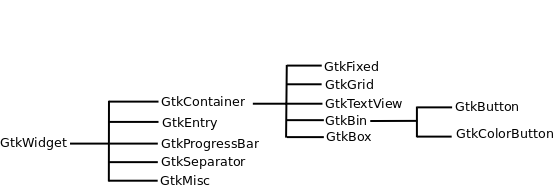
\includegraphics[scale=0.7]{../images/dia/arbo_widget.png} 
        \caption{Arborescence des Widgets les plus utilisés dans Beeterface}
        \label{arbo_widg}
\end{figure}
Par exemple, je veux changer un paramètre d'un élément "GtkSpinButton". Malheureusement, je ne trouve pas de fonction 
affectant directement ce paramètre, par exemple la taille. Alors je vais regarder si chez ses parents, je peux trouver 
le paramètre voulu, à savoir chez "GtkEntry", et "GtkWidget". \\
Chaque paramètre disponible pour les Widgets peut être changé directement à l'aide de fonctions retrouvable dans la très complète 
documentation en ligne de GTK 3.0. Il est totalement déconseillé de changer directement la valeur des paramètres à la main 
en utilisant les pointeurs. Il faut partir du principe que chaque élément a son nombre de fonctions associées 
et que tout est prévu pour pouvoir faire ce que l'on veut sur notre interface. \\ 

        \subsection{Des boites, dans des boites...}
Une fois la façon dont les éléments et leurs paramètres sont gérés acquise, il faut ensuite pouvoir les ranger. 
D'abord, on va créer une fenêtre, soit une "GtkWindow" que l'on va appeler Window. Dans celle-ci, on ne peut y poser qu'un seul Widget. 
C'est pour ça que nous avons les éléments "GtkContainers" : ce sont ces containers que nous allons pouvoir structurer et placer tous 
les autres éléments comme on le veut dans notre fenêtre. \\
Le GtkContainer de base est la "GtkBox". À sa création, nous devons simplement indiquer si celle-ci va être horizontale ou verticale, 
c'est à dire si les éléments que nous allons mettre dedans vont être placés de haut en bas ou de gauche à droite. 
Une fois cette première "GtkBox" placée, le problème de limitation de place imposée par la "GtkWindow" n'en est plus un. 
Maintenant, nous pouvons ranger ce que nous voulons dans cette boite. C'est là que le système de poupée russe prend son sens : 
nous allons devoir jouer avec les différentes boîtes pour créer les espaces que nous désirons. 
Pour se faire une idée, j'ai réalisé un schéma de placement de ces boites pour la fenêtre principal, win\_main 
\footnote{Voir Figure \ref{sch_box_win_main}}.
\begin{figure}[!h]
    \centering
        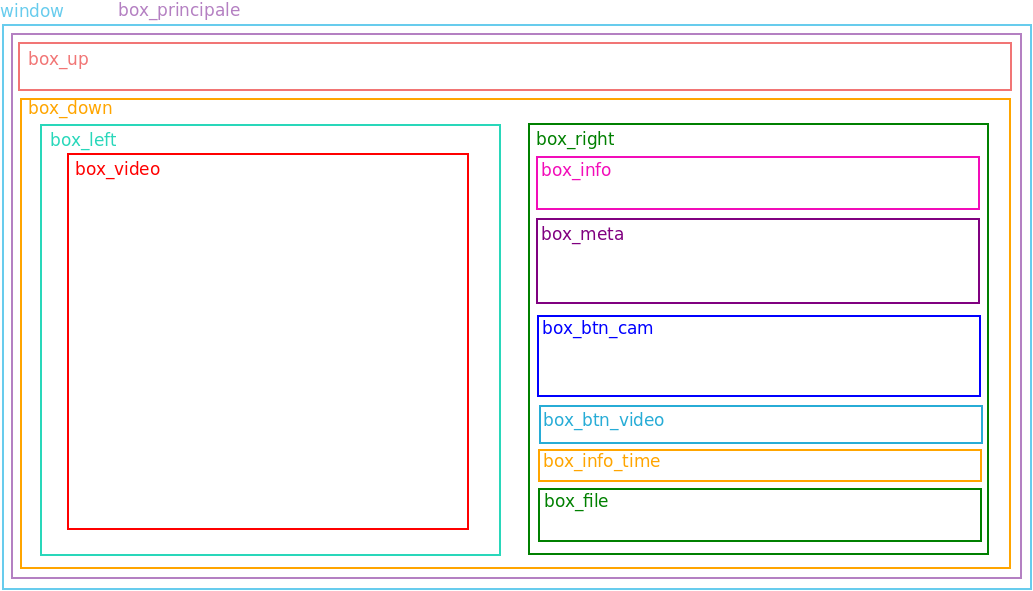
\includegraphics[scale=0.5]{../images/dia/schema_bloc_mainwin.png} \\
        \caption{Schéma de placement des box pour win\_main}
        \label{sch_box_win_main}
\end{figure}
On peut voir que la "GtkBox" box\_principale prend toute la place de ma fenêtre "GtkWindow". Dans cette box\_principale, j'y ai rangé 
verticalement box\_up et box\_down. Dans box\_down j'ai intégré box\_left et box\_right horizontalement, me permettant d'avoir 
quatre zones délimitées. \\
Ensuite, j'ai créé des box pour mes éléments plus précis : dans box left j'ai directement placé box\_video dans laquelle 
se trouve la vidéo (pour le moment, une image fixe représentant là où la vidéo se trouvera par la suite). 
Dans box right on va retrouver box\_info, box\_meta, box\_btn\_cam, box\_btn\_video, box\_info\_time et box\_file. 
Chacune de ces box m'a permis de ranger à l'intérieur les éléments que je voulais retrouver : 
les boutons, les textes, les descriptions, etc. 
À noter qu'en plus de ces "GtkBox" j'ai également utilisé d'autres types de "GtkContainer". Des "GtkFrame", l'encadrement
avec un titre autour d'"Informations Capteurs" et "Informations Vidéo". Des "GtkGrid", permettant de placer les éléments 
à la manière d'un tableau sans les bordures, ici utilisé pour le texte dans les deux encadrés "Informations". \\
Un autre type de Gtkcontainer intéressant que je n'ai pas utilisé ici est le "GtkScrolledWindow". Celui-ci permet d'ajouter
une barre de défilement afin d'afficher plus d'informations. \\
Le résultat nous donne l'impression de ne pas voir toutes les boites clairement \footnote{Voir figure \ref{res_box_win_main}}. \\
\begin{figure}[!h]
    \centering
        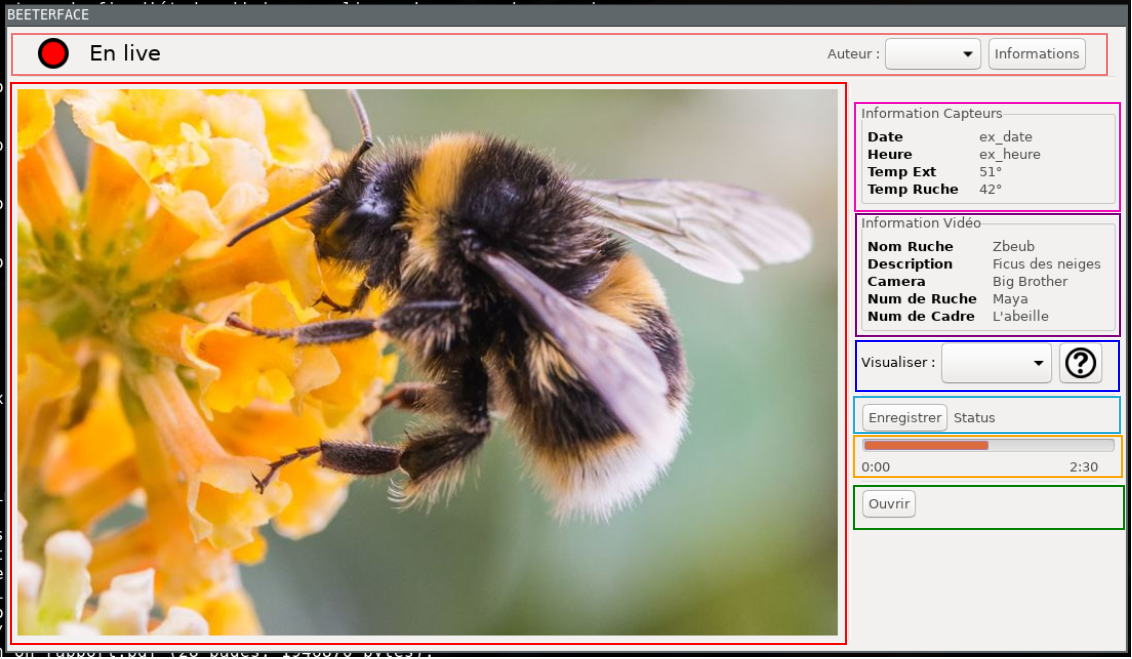
\includegraphics[scale=0.45]{../images/dia/schema_bloc_win_applique.png} \\
        \caption{Résultat du placement des box pour win\_main}
        \label{res_box_win_main}
\end{figure}
C'est dû au fait que les boites prennent toute la place qu'elle peuvent en fonction des widgets qu'elles contiennent. Ainsi, box\_principale 
n'est pas clairement visible : elle ne sert que de support pour les autres "GtkContainers". 
Maintenant que nous avons les deux principes de bases en tête, à savoir les éléments et les boîtes, on peut voir comment 
tout cela se forme dans le code. \\
GTK nécessite une organisation rigoureuse si on veut pouvoir s'y retrouver avec les éléments rapidement nombreux.
Ainsi, j'ai voulu identifier les différentes étapes de la création d'un Widget et les séparer en 
trois grandes parties pour m'y retrouver plus facilement. \\

        \subsection{Création et Définition}
La première chose à faire est de créer les Widgets et de les définir. La création est simplement la déclaration d'une variable 
avec son type. 

\dotfill \\
Appartée
Avant toute chose, notons que j'utilise des pointeurs pour toute mon application et que mes exemples 
sont inspirés des fichiers win\_main.c et win\_main.h disponibles en annexes 
afin que vous puissiez vous y reporter pour voir des exemples plus complets et concrets. 
La structure en .c/.h et l'explication des pointeurs utilisés sont décrits dans la partie "Les structures" de 
"Définition des fonctionnalités". Pour le moment, ne prenons pas en compte les "tmp->" placés devant les noms des éléments.
Ils permettent juste d'indiquer que nous sommes dans la définition de la fenêtre win\_main.
De plus, les noms utilisés (label, box et window) n'existent pas dans win\_main. Ils ont été simplifiés ici, 
mais leurs équivalents sont facilements retrouvables dans win\_main.\\
\dotfill \\

Créons une fenêtre, une box et un label.\\
\small Dans win\_main.h : \normalsize
\begin{lstlisting} [frame=single]
GtkWidget* window ; 
GtkWidget* box ;   
GtkWidget* label ;  
\end{lstlisting}
Ici, les éléments sont tous du type "GtkWidget", ce sera le cas pour la majorité de nos éléments lors de la 
déclaration.
Il arrive que, dans de rares cas, il soit nécessaire de les déclarer autrement : si c'est le cas, la documentation l'indiquera. \\ 
Désormais, ces trois élément existent. Maintenant il faut les définir, c'est-à-dire expliquer de quel type de Widget ils sont 
et leur donner leurs propriétés. \\
\small Dans win\_main.c : \normalsize
\begin{lstlisting} [frame=single]
tmp->window = gtk_window_new (GTK_WINDOW_TOPLEVEL) ;
\end{lstlisting}
Ici, on utilise la fonction "gtk\_window\_new" pour indiquer que "window" est une fenêtre qui s'ouvre en premier plan 
avec l'argument "GTK\_WINDOW\_TOPLEVEL". \\
\small Dans win\_main.c : \normalsize
\begin{lstlisting} [frame=single]
tmp->box_principal = gtk_box_new( GTK_ORIENTATION_VERTICAL, 0) ;
\end{lstlisting}
Comme dit plus haut, à la création d'une "GtkBox" on indique d'abord si on veut que les éléments soient ajoutés verticalement 
ou horizontalement. Le second argument permet de définir le nombre de pixels d'écart par défaut entre les éléments, 
ici 0px, donc ils seront collés l'un à l'autre.  \\
\small Dans win\_main.c : \normalsize
\begin{lstlisting} [frame=single]
tmp->label = gtk_label_new("Je suis le texte du label") ; 
\end{lstlisting}
Le label nécessite lui aussi un argument, ici ce sera le texte qu'il affichera. 
On peut laisser ce texte vide si on ne remplit pas les "".  \\
Les exemples ci-dessus ont tous eu besoin d'une définition précise du Widget, avec à chaque fois au moins un paramètre à régler. 
Il arrive parfois que la création ne nécessite aucun paramètre, et que des modification doivent être apportées ensuite. 
Par exemple, si je veux que mon label ait une écriture plus stylisée, je peux utiliser :  \\
\small Dans win\_main.c \normalsize
\begin{lstlisting} [frame=single]
gtk_label_set_markup(GTK_LABEL(tmp->label), 
                    "<span foreground=\"black\" font=\"10\"><b>Je suis le label stylisée avec du bold</b></span>"); 
\end{lstlisting}
Ici, avant d'indiquer quel élément on veut modifier, il faut préciser de quel type d'élement il s'agit.
En effet, comme lors de la déclaration il est indiqué que le label est de type GtkWidget et que la fonction que l'on veut utiliser 
ne s'applique que sur un GtkLabel, il est donc nécessaire de "forcer" GTK à considérer "tmp->label" comme un label.\\
Il existe plein de fonctions différentes permettant de régler ce genre de paramètres sur les widgets, et il est parfois nécessaire 
de faire appel à elles pour avoir un Widget correct. 
Il est intéressant d'explorer les fonctions existantes afin de personnaliser au mieux notre interface. \\
Une fois les Widgets créés, il faut maintenant les placer et indiquer qu'il faut les afficher. \\ 

    \subsection{Placement et affichage} \\
Maintenant, nous allons appliquer ce qui a été expliqué plus haut pour placer les éléments. On va commencer par dire où 
va se placer la box : \\
\small Dans win\_main. \normalsize
\begin{lstlisting} [frame=single]
 gtk_container_add (GTK_CONTAINER (tmp->window), tmp->box) ; 
\end{lstlisting}
GtkWindow hérite de GtkContainer, nous utilisons donc la fonction qui permet d'affecter un élément à un container. Le premier argument 
indique le container où nous devons insérer un élément. Le second nous indique quel élément est à placer. \\
Ensuite, nous faisons de même pour la box : \\
\small Dans win\_main.c
\begin{lstlisting} [frame=single]
gtk_box_pack_start(GTK_BOX(tmp->box_principal), tmp->label, FALSE, FALSE, 0) ; 
\end{lstlisting}
"box\_principal" étant de type GtkBox, nous utilisons cette fois la fonction qui lui est associée. 
Comme pour "window", il faut indiquer la boîte concernée par l'élément à ajouter, mais cette fois-ci trois autres arguments 
sont à renseigner concernant la manière dont les Widgets vont se comporter à l'intérieur de la box. \\ 
Il faut savoir que par défaut les box allouent la même place à tous les Widgets qu'ils contiennent
sans déborder sur le reste.\\
\begin{itemize}
    \item Expand : peut être TRUE ou FALSE. Permet aux widgets de prendre plus de place si besoin si réglé sur TRUE. 
    \item Fill : peut être TRUE ou FALSE. Ne peut être actif que si Expand est aussi TRUE. Alloue la hauteur ou la largeur totale
        de la box, 
        celon si la box est une horizontale ou vertical.
    \item Padding : valeur numérique. Indique l'espacement en pixel (px) entre les widget que contient la box. 
\end{itemize}
Les éléments sont maintenant placés. Afin d'avoir une relecture facile et pour savoir qui se trouve dans quelle box ou container, 
j'ai appliqué une indentation  qui m'est propre mais que je trouve plus lisible. L'exemple pour main\_win.c est disponible en annexe
\footnote{Voir Annexes \ref{3} et \ref{4}}. 
Ainsi, à chaque fois que je place un élément dans une nouvelle box contenue elle-même dans une box, j'indente avec une 
tabulation. Le rendu me permet de voir qui est à quel niveau. \\
Petite précision, les éléments seront placés dans l'ordre de lecture du code. Ainsi, si votre "GtkBox" est créée en tant
que box horizontale, l'élément placés en premier sera le plus à gauche, le suivant à sa droite et ainsi de suite. \\ 
Le diagramme de placement des Widget \footnote{Voir figure \ref{org_win_main}} permet de voir cette 
indentation schématiquement pour visualiser ce principe de "poupées russes".
\begin{figure}[!h]
\centering
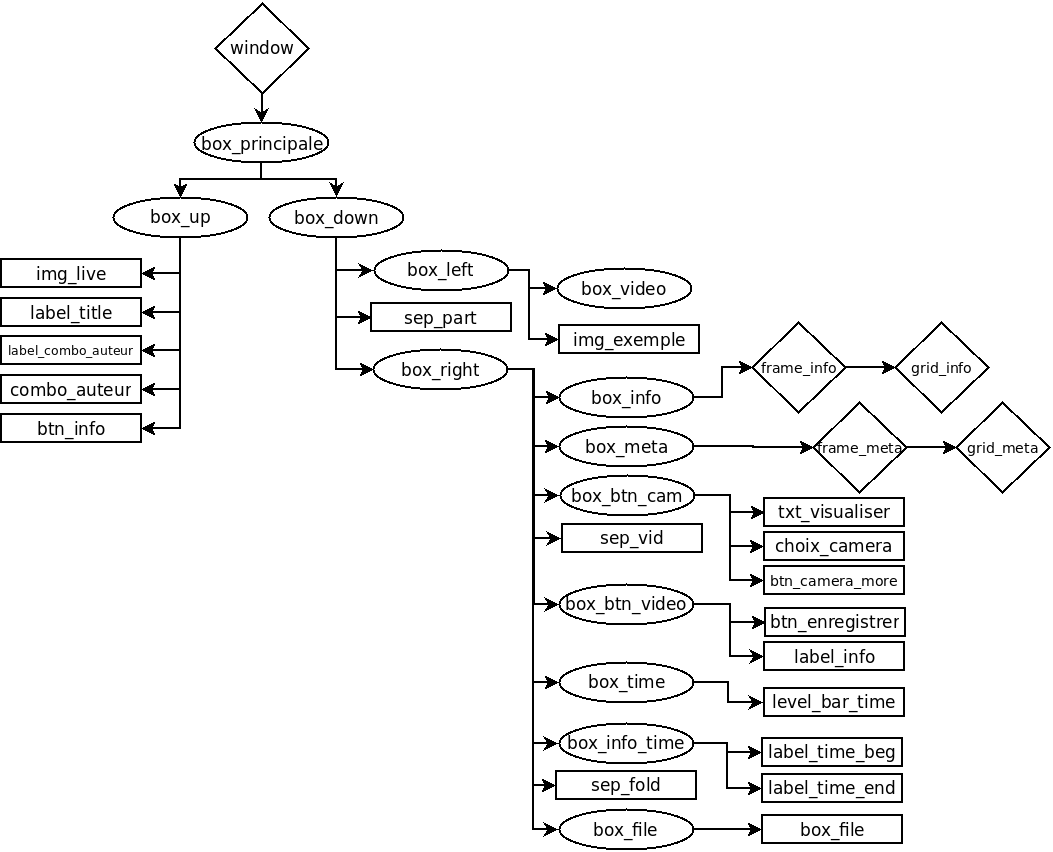
\includegraphics[scale=0.5]{../images/dia/diagramme_fenetre.png} 
        \caption{Diagramme des Widgets pour win\_main}
        \label{org_win_main}
\end{figure}
Une fois que les éléments sont placés dans les boîtes, ceux-ci sont tous collés les uns aux autres ou avec 
les espaces de bases indiqués lors de la création des box. 
Il faut indiquer comment ils doivent se placer. Pour mieux comprendre ce que nous allons faire, il faut voir un 
avant/après les fonctions que je vais présenter \footnote{Voir figure \ref{avap}}.

\begin{figure}[!h]
    \centering
    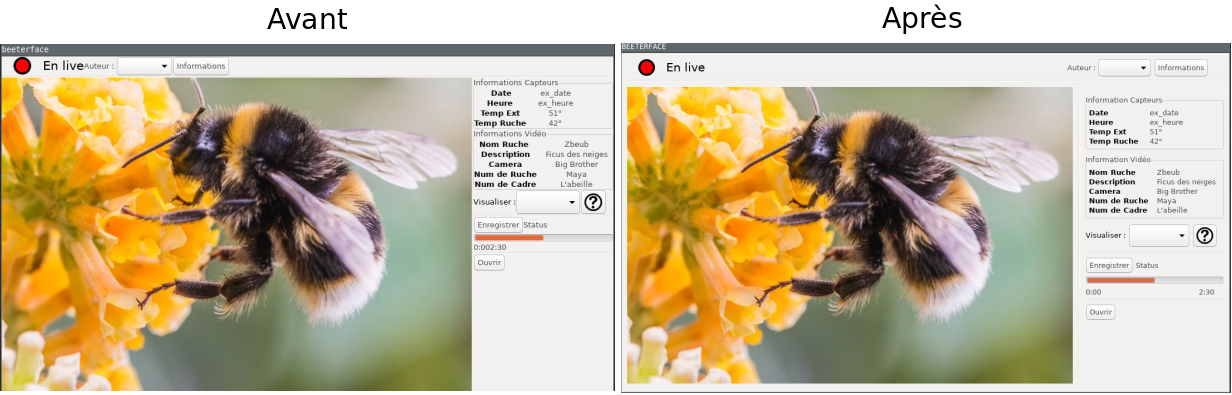
\includegraphics[scale=0.4]{../images/annexes/av_ap.png} 
    \caption{Avant/Après un meilleur placement}
    \label{avap}
\end{figure}

Tout d'abord, commençons par jouer avec les paramètres EXPAND et FILL des "GtkBox". Ils permettent de définir quels éléments seront 
autorisés à s'agrandir en même temps que la fenêtre. Le mieux pour bien comprendre leur comportement, c'est de tester au fur
et à mesure les différentes combinaisons expliquées plus haut. \\
Comme pour la création et le placement, nous allons utiliser des fonctions pour indiquer ce que l'on veut faire avec les éléments.
Ce type de fonction est utilisé sur les éléments de types "GtkWidget", et donc applicable sur tous ceux qui en héritent. Voici les
deux fonctions et leurs variables que j'ai le plus utilisé : \\
\begin{lstlisting} [frame=single]
 gtk_widget_set_margin_top (GTK_WIDGET (tmp->label), 5 ) ; 
\end{lstlisting}
Permet d'appliquer une marge sur le haut. On précise sur quel Widget l'appliquer puis la taille en px de la marge.
Cette fonction existe aussi pour bottom, end et start qui correspondent au bas, à la droite et la gauche du Widget
\footnote{Voir figure \ref{sch_pla_top}}.\\
\begin{figure} [!h]
    \centering
        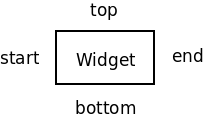
\includegraphics[scale=0.5]{../images/dia/top_bottom_etc.png}
        \caption{Schéma du placement de start, end, top, bottom}
        \label{sch_pla_top}
\end{figure}
\begin{lstlisting} [frame=single]
 gtk_widget_set_halign ( GTK_WIDGET (tmp->label), GTK_ALIGN_START ) ;
\end{lstlisting}
Les éléments se mettent par défaut au centre de leur place disponible. Cette fonction permet 
de forcer un Widget à se placer autrement : ici, on force l'alignement horizontal (halign) à être en début de zone, 
soit à gauche (START). \
On peut aussi retrouver des fonctions pour préciser le comportement de la fenêtre, comme :
\begin{lstlisting} [frame=single]
gtk_window_set_title (GTK_WINDOW (tmp->window), "BEETERFACE") ; 
\end{lstlisting}
qui permet de nommer la fenêtre "BEETERFACE". \\
\begin{lstlisting} [frame=single]
gtk_window_set_default_size ( GTK_WINDOW (tmp->window), 30, 30 ) ; 
\end{lstlisting}
Définit la taille minimale de la fenêtre, sachant qu'elle prend en compte la place nécessaire aux éléments pour pouvoir 
être placés et que si la taille indiquée est trop petite, alors la fenêtre prendra la place minimale possible 
pour afficher les éléments. \\
Avec ces outils et un peu de recherches sur la documentation en ligne, on peut maintenant créer n'importe qu'elle fenêtre 
comme on le souhaite. 
Attention, à cette étape nous avons juste définit l'interface. Il reste encore une étape pour pouvoir afficher les éléments, sinon
les éléments seront créés, placés... Mais invisibles ! 
Personnelement, j'aime la faire en deux étapes. D'abord l'affichage de la fenêtre avec : \\
\begin{lstlisting} [frame=single]
gtk_widget_show (tmp->window) ;
\end{lstlisting}
Puis de la box principale avec tout ce qu'elle contient : \\
\begin{lstlisting} [frame=single]
gtk_widget_show_all (tmp->box_principal) ; 
\end{lstlisting}
Sachant que l'affichage se fera dans l'ordre annoncé, si vous avez peur que le logiciel apparaisse "étape par étape", c'est à 
dire avec les éléments apparaissant au fur et à mesure laissant au début une fenêtre vide restant affichées quelques secondes, 
préférez mettre l'affichage de la box principale avant l'affichage de la fenêtre. Ainsi, la box et ses enfants seront déjà générés 
et n'auront besoin que de leur support, soit la window. Cependant, cette question se pose uniquement si l'application 
à afficher nécessite beaucoup de ressources. \\
Notre interface est désormais prête \footnote{Voir Annexe \ref{an2} }
il ne reste plus qu'à lier des fonctions aux différents éléments pour que notre application soit utilisable.\\
        
        \subsection{Signaux et fonctions} 
Avoir des boutons, c'est bien. Pouvoir les utiliser, c'est encore mieux. Maintenant que tous éléments sont placés, 
il ne reste plus qu'à les lier aux fonctions qui permettront de réaliser diverses tâches (mettre en pause la vidéo,
se déplacer dans le temps de celle-ci, débuter la sauvegarde etc).    
C'est ce qui va établir le lien entre le moteur et la carcasse. \\
Pour le moment, peu de fonctions ont été écrites pour le moteur : toute la partie graphique est prête à les accueillir 
mais le développement des fonctionnalités est ce qui prend le plus de temps. En guise d'entraînement et pour 
pouvoir être prête le jour où il faudra faire tous les liens, j'ai déjà fait quelques tests pour comprendre les principes.
Les liens entre l'interface et les fonctions vont se passer dans le main. Dans notre code, il est présent dans beeterface.c 
\footnote{Voir en Annexe \ref{an3}}.\\
Avant tout, il faut noter que quelques fonctions sont obligatoires pour le bon fonctionnement de GTK. Les voici : \\
\begin{lstlisting} [frame=single]
int main(int argc, char *argv[])     
{ 
 gtk_init(&argc, &argv); 
 [votre code] 
 gtk_main();
 return 0 ;
} 
\end{lstlisting}
Ces deux fonctions permettent d'initialiser l'interface et d'indiquer que celle-ci est en attente de signal
de la part de l'utilisateur pour réagir. \\
Maintenant que nous avons la base, commençons à intégrer des événements.
Le but va être d'appeler une fonction GTK qui va lier un élément à une autre fonction que nous avons écrit  (Callback) 
et d'indiquer en quelle circonstance la callback doit s'activer. Voici ladite fonction : 
\begin{lstlisting} [frame=single]
g_signal_connect( queen->interface->win_main->btn,
                   "clicked", 
                    G\_CALLBACK(callback_btn) ,
                    queen ) ; 
\end{lstlisting}
Le premier argument correspond à l'élément qui est visé. Dans notre cas, beaucoup de pointeurs sont en jeu,
pour le moment nous allons passer outre ces pointeurs : ils seront expliqués dans la partie structure. 
Partons simplement du principe qu'il faut appeler le bouton ou élément concerné, ici btn.  
Le second argument sert à indiquer à quel événement il faut réagir. Il en existe une liste prédéfinie : ici,
c'est l'événement "clicked". Lorsqu'on cliquera sur le bouton, la callback sera appelée. 
Le troisième argument correspond à la "callback" appelée, soit la fonction qui doit se déclencher. Nous allons 
y revenir.
Le dernier argument indique ce qu'on envoie aux callbacks comme information. Ici, c'est "queen", une sorte de 
gros paquet. Comme pour les pointeurs, ce sera expliqué plus tard. \\
void callback_quit_tag(GtkWidget* widget, gpointer data) {                                       
    queen_t* tmp ;                                                                             
    tmp = data ;                                                                                
    gtk_window_close (GTK_WINDOW(tmp->interface->win_main->window)) ; 
} 
\end{lstlisting}
Cette callback contient le strict minimum pour faire fonctionner simplement un bouton.
En arguments, elle reçoit d'abord le widget qui est à la source de son appel : dans notre cas, c'est "btn". 
Ensuite, elle reçoit les data que "g\_signal\_connect" a envoyé, c'est-à-dire "queen". \\

Les deux premières lignes indiquent que la variable tmp reçoit les informations de data. 
Enfin, la fonction utilisée permet d'indiquer qu'on va fermer une fenêtre, ici celle de win\_main, donc là où on
se trouve. Cet exemple est basique, on peut évidemment faire bien plus et toucher à l'interface en elle-même, déclencher
d'autres fonctionnalités, ouvrir de nouvelles fenêtres, modifier des informations...\\

Tous les outils principaux pour pouvoir créer une interface GTK ont été présentés. Avec ceux-là, beaucoup de recherches
dans la documentation et le "catalogue"
de GTK, on a en mains une infinité de possibilités. Certaines actions nécessitent plus de réflexion que d'autres, mais 
au final ça n'est que de l'algorithmie ; toute la syntaxe est là. \\


    \section{Les fonctionnalités} 
        \subsection{Structuration du code}
La première chose que j'ai eu à faire pour la création de l'application a été de réfléchir à la façon dont elle allait fonctionner.
En étudiant la demande, une chose majeure en ressortait : il y allait avoir beaucoup de type de données à traiter et sauvegarder. \\
Si on lit la liste des besoins présentés dans la partie 2.1
on peut voir qu'il y a, entre autres, une notion d'auteur, de caméra, de vidéo et de ruche.

Afin de pouvoir manipuler de telles informations, j'ai créé une structure (struct en C) pour chacun des éléments nécessaires. \\
Ils contiendront chacun des informations nécessaires à leur fonctionnement : dates, noms, numéro de téléphone, lieu, référence, etc. \\

Par exemple, voici la définition de la structure "author" : 
\begin{lstlisting} [frame=single]
typedef struct {
char* lastname;
char* firstname;
char* email;
} author_t ;

author_t* author_new() ;
void author_del (author_t*);
void author_show (author_t*);

void author_set_lastname( author_t* , char* lastname ) ;
char* author_get_lastname ( author_t* ) ;

void author_set_firstname( author_t* , char* firstname ) ;
char* author_get_firstname ( author_t* ) ;

void author_set_email( author_t* , char* email ) ;
char* author_get_email ( author_t* ) ;
\end{lstlisting}

Pour chacune des structures, j'ai également préparé des fonctions permettant de manipuler les données.
En général, on y retrouve une fonction pour créer un élément (new\_element), une pour le supprimer (del\_element),
et un jeu de fonction pour modifier (set\_partie\_element) ou lire les données contenues dans l'élément indépendamment 
(get\_partie\_element). L'exemple pour author.c est en Annexe \footnote{Voir Annexe \ref{an6}}.\\

Cette préparation permettra de pouvoir utiliser ces données sans avoir à se soucier des pointeurs : tout est prêt, il n'y
a plus qu'à choisir comment on voudra modifier les données lors de l'utilisation du logiciel. \\

Ce travail a aussi été fait pour toutes les annotations que nous pourrons intégrer sur les vidéos : 
les cercles, flèches, croix... \\

Pour le moment, toutes ces annotations ne sont pas prêtes. Mais les plus basiques, comme la croix, ont déjà leur structure de préparées.
Sa définition se fait avec un simple x et un y. D'autres nécessitent d'autres indications, comme un angle pour la flèche
ou un tableau de coordonnées pour la croix mouvante. \\
En plus des descriptions des éléments, tous contiennent un champ nom, auteur, couleur, description, temps de début 
(quand il apparaît sur la vidéo) et temps de fin (quand il disparaît de la vidéo). 
On peut aussi faire mention du champ "tag[]" et "tag\_size" qui correspondront à une pile de tag qui est affecté à l'élément. \\
C
ajouter facilement des nouveaux tags. Les tags pourront être affectés aux différentes annotations appliquées
à une vidéo, et cette vidéo héritera de ces tags dans sa description, nous permettant de trier et récupérer les vidéos 
en fonctions de ce qu'il s'y trouve. \\
Concernant sa définition, un tag sera décrit par une pile. À ce niveau, il reste encore quelques précisions à apporter
avant de la coder. Cette tâche est pour le moment en attente dans notre TO DO LIST.\\
Ce travail de préparation m'aura pris environ une semaine. Il a été difficile seulement au début : il fallait réfléchir 
la manière de créer une structure correctement, penser à bien utiliser les pointeurs et gérer leur allocation de
mémoire. Une fois un premier modèle fait, les autres se faisaient de plus en plus vite. Utilisant l'éditeur de texte VIM, j'ai 
énormément utilisé les "rechercher/remplacer" pour travailler. \\
Ce travail, bien que fastidieux, m'aura permis d'appliquer concrètement l'utilisation des pointeurs, ce qui 
me manquait lors de mon arrivée en stage. \\ 

        \subsection{Manière de coder}\\
N'ayant pas d'habitudes particulières en code, j'ai été conseillée pour le structurer, afin qu'il 
soit facilement lisible. Ainsi, j'ai utilisé des couples de fichiers .c et .h me permettant de séparer 
la déclaration d'une structure et de ses fonctions et la définition des fonctions.

De plus, M. Druon a rapidement intégré un Makefile afin de nous éviter de compiler manuellement à chaque fois, passant 
ensuite à CMake pour générer le Makefile automatiquement ensuite. \\
Une fois cette façon de faire mis en place pour la partie moteur, j'ai voulu l'appliquer à la partie
graphique. Ainsi, un couple de .c et .h a aussi été créé pour chacune des fenêtres, le .h contenant 
toutes les déclarations d'éléments sous forme de structure \footnote{Voir Annexes \ref{3} et \ref{4}}. \\

Dans le .c on retrouve la fonction de création de l'interface avec au début la définition de "tmp" qui correspond donc 
au "papier cadeau" contenant toutes les déclarations des éléments. 

C'est pourquoi nous avons vu sur les exemples plus haut 
que pour appeler un élément nous devions utiliser un pointeur comme "tmp->label". \\

Notre fichier .c contient alors de quoi créer l'interface, l'afficher et la supprimer, la suppression revenant à appliquer les 
Free  nécessaires. C'est pour cela que dans notre "main", on retrouve ces fonctions pour définir et afficher les fenêtres 
et que celui-ci est allégé. \\

Jusque-là, cette technique m'a permis d'avoir une structure de code agréable et ordonnée. Seulement, une fois arrivée au moment de 
faire les premiers liens interface / fonctions qu'un autre problème s'est posé : comment pouvoir accéder à toutes les données
dont j'ai besoin lorsque j'utilise une callback ? 
Comme dit dans la partie 2.2.5, lorsqu'on appelle une callback quand événement est détecté, deux informations sont 
transmises à la callback : l'adresse du Widget et une data qui aura été définie avec la fonction "g\_signal\_connect". \\

C'est le choix de cette donnée qui nous a posé problème : quand nous avons commencé
à coder les fenêtres permettant la visualisation des données des auteurs, caméras etc, nous avions besoin d'envoyer la structure
de la fenêtre auteur par exemples mais aussi les informations de l'auteur, ne se trouvant pas dans les mêmes fichiers.  \\
La solution la plus simple était donc de refaire des "paquets" plus généraux : nous avons créé interface.c/h et projet.c/h, qui seront eux
même contenu dans queen.c/h. \\
"Interface" contient toutes les fenêtres possibles et a une fonction de créations de toutes celles-ci ainsi qu'une fonction de suppression, 
permettant de les créer au démarrage de l'application et éviter des chargement. La fonction de suppression nous assure d'éviter toute perte de mémoire.\\
Même principe pour le Projet : il contient tous les éléments permettant le fonctionnement moteur afin d'avoir la même facilité
d'utilisation que décrite pour l'interface. \\
Queen est le paquet général, il contient Interface et Projet. Son nom est en l'honneur de la reine des abeilles : 
un paquet pour les gouverner tous ! \\
Afin de vérifier que toute cette structure soit cohérente et pour l'améliorer, Mr Druon a réalisé un diagramme 
avec toutes les structures \footnote{Voir figure \ref{dia_struct}}.
\begin{landscape}
\begin{figure}[!h]
    \centering
    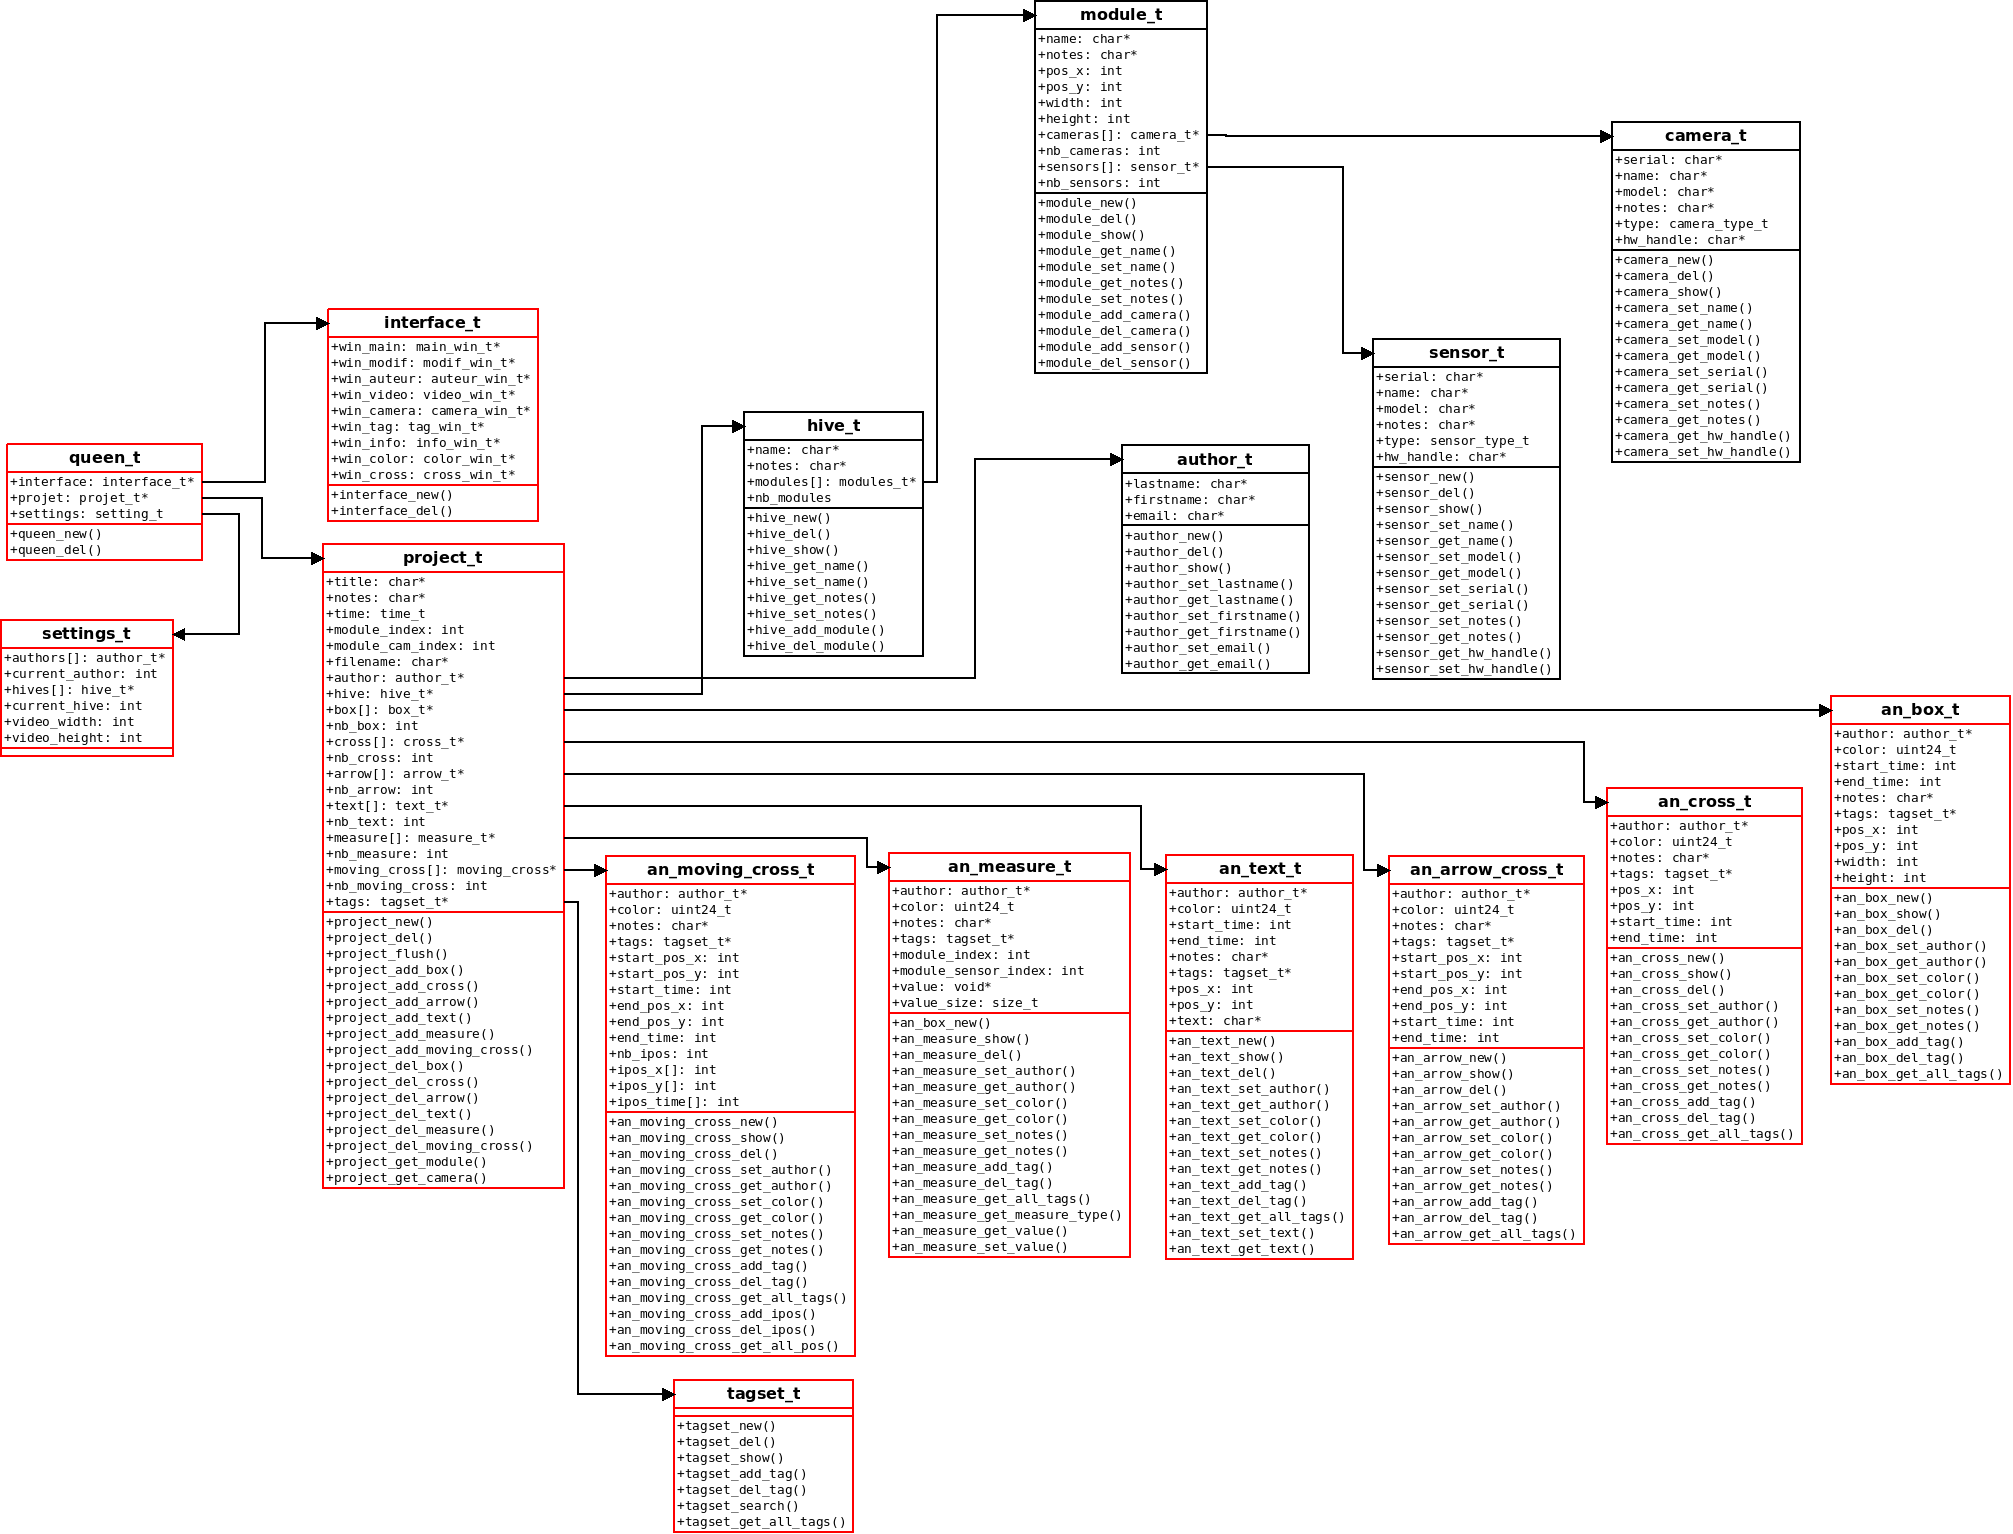
\includegraphics[scale=0.3]{../images/dia/beeterface_structs.png}
    \caption{Diagramme des structure de Beeterface}
    \label{dia_struct}
\end{figure}
\end{landscape}
Et voici un bout de code représentant ce que l'on peut faire avec les paquets : 
\begin{lstlisting}
callback\_auteur(GtkWidget * widget, gpointer data)
 {
     queen\_t* tmp ;
     tmp = data ;
     // Remplissage de la fenêtre avec le contenu de auteur
     auteur\_win\_fill(tmp->interface->win\_auteur, tmp->projet->video->auteur ) ;

     auteur\_win\_show(tmp->interface->win\_auteur);
 }
 void callback\_auteur\_modify\_name(GtkWidget* widget, gpointer data) {
         queen\_t* tmp ;
         tmp = data ;

         if ( tmp->interface->win\_auteur->button\_modif\_1 == 0 )
         auteur\_button\_modify\_name(tmp->interface->win\_auteur, tmp->projet->video->auteur ) ;
         else
         auteur\_button\_modify\_ok\_name(tmp->interface->win\_auteur, tmp->projet->video->auteur ) ;
   }
\end{lstlisting}
Dans cet exemple, on retrouve la fonction "auteur\_win\_fill", fonction écrite dans win\_auteur\_callbacks.c et définie
dans win\_auteur.h. J'ai séparé les fonctions utilisées dans les callbacks afin de les retrouver facilement. \\
Voici donc comment le projet a été réflechi et construit. Normalement, avec ces détails, un développeur qui voudrait reprendre
le projet pourrait retrouver les données facilement. Dans cette optique, nous avons également prévu d'utiliser
l'utilitaire Naturaldocs afin de documenter le code, quelques exemples sont d'ailleurs déjà présents, mais la documentation 
complète n'était pas une priorité, c'est pourquoi cette tâche a été laissée en suspens. 
       
        \subsection{Traitement de la vidéo}
La partie la plus complexe de ce projet à mon avis est le traitement de la vidéo. Elle s'attaque à des sujets sur lesquels j'ai 
encore beaucoup à apprendre. C'est pourquoi durant le stage, c'est plus M. Druon qui s'en est occupé. De mon côté, j'ai surtout
pris en compte ce qui allait être fait avec et ce que j'allais devoir prévoir au niveau de l'interface pour que cela fonctionne. \\
Globalement, l'idée de ce travail est dans un premier temps d'afficher la vidéo sur l'application grâce à 
la librairie FFMPEG. Afin de me faciliter
le travail de lien entre les boutons et la vidéo, M. Druon a prévu de créer plusieurs fonctions type, comme avancer la vidéo, la 
mettre en pause, la reculer, pour qu'ensuite elles soient affectées à l'interface. \\
Dans un second temps, il faut pouvoir enregistrer la vidéo une fois qu'elle est annotée. L'idée est de faire en sorte que les annotations
soient des PNG appliqués au-dessus de l'image et qu'ils soient transportés dans les mêmes flux que les flux vidéos. \\

Ce travail a été commencé durant mon stage et devrait être fini aux alentours de septembre. C'est pourquoi sa description ici
est surtout théorique. \\
        \subsection{Ce qu'il reste à faire}
Une application prenant du temps à être développée, il est normal que celle-ci n'ait pas été finie en 3 mois. Pour pouvoir se situer
dans l'avancement de ce projet, j'ai établi une liste non-exhaustive de ce qui, à l'heure actuelle, resterai à faire : \\ 
\begin{itemize}
    \item Établir le système de sauvegarde des données.
    \item Configurer la façon dont les données seront envoyées sur le serveur (fréquence d'envoi, envoi automatique ou manuel etc).
    \item Coder la façon dont les tags vont être gérés pour le tri des vidéos. 
    \item Continuer l'affichage vidéo.
\end{itemize} 
De manière plus personnelle, j'aurais également aimé pouvoir retravailler la structure interne de beeterface.c qui est, à mon sens,
un peu brouillon. \\
Pour finir cette présentation de l'application, voici quelques screenshots du travail qui a été effectué.
Le travail fut long et n'a cessé d'évoluer : au fur et à mesure, j'aurai appris de nouvelles techniques, de nouvelles façon de faire 
et aurais profité de nombreux conseils d'un développeur senior. \\

\chapter{Acquis et compétences}
Ce stage m'aura permis d'utiliser mes compétences acquises pendant le DUT, mais aussi d'en développer d'autres grâce aux activités 
que j'ai réalisé. Pour chaque missions, que ça soit la principale ou les annexes, j'ai pu apprendre sur une multitude de domaines
différents : techniques, théoriques, humains, organisationnel, etc. 
Ainsi, la présentation des missions annexes et la liste des domaines où je sens que j'ai évolué semblent être un bon moyen 
de présenter tous ces acquis. 
\section{Missions annexes}
        
        \subsection{Gestion du Réseau du Rucher}
Le projet se basant sur du traitement et de la récolte de données, une infrastructure réseau est à prévoir 
\footnote{Voir figure \ref{plan_res}}. Pour le moment, nous avons surtout préparé le terrain.  \\
Les données seront récoltées au rucher, puis acheminées vers le serveur installé au CNRS. Ce serveur les stockera et les traitera, 
les envoyant à différents endroits selon le besoin : vers les applications Beeterface pour de l'annotation, vers la future vitrine Web
etc. \\
Seulement, à mon arrivée, il n'était pas encore raccordé au réseau : tout le long de mon stage,  nous avons dû attendre que
le CNRS nous installe la fibre. \\
\begin{figure}[!h]
    \centering
    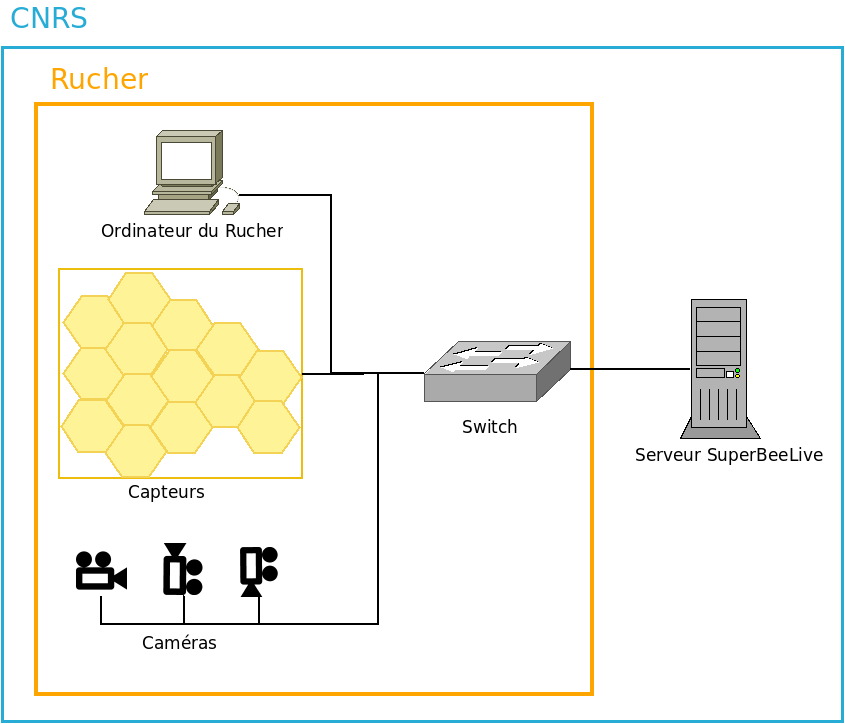
\includegraphics[scale=0.3]{../images/dia/plan_reseau.png}
    \caption{Plan prévisionnel du réseau}
    \label{plan_res}
\end{figure}
Même si un biologiste annotait les vidéos avec Beeterface directement au rucher, les vidéos devront obligatoirement passer une première 
fois vers le serveur puis revenir au rucher. Ainsi, entre l'envoi de vidéos venant de caméras pouvant atteindre de hautes
qualités et la réception de ces mêmes vidéos, la bande passante et le matériel réseau installé sur place 
doivent pouvoir supporter de telles charges. \\
C'est pourquoi le technicien s'occupant de l'installation de la fibre devait connaître quel trafic était prévu de manière un
peu plus détaillée. Afin de répondre à cette question, nous avons effectué un récapitulatif des caméras prévues 
\footnote{Voir figure \ref{tab_recap_cam}}
\begin{figure}[!h]
    \centering
    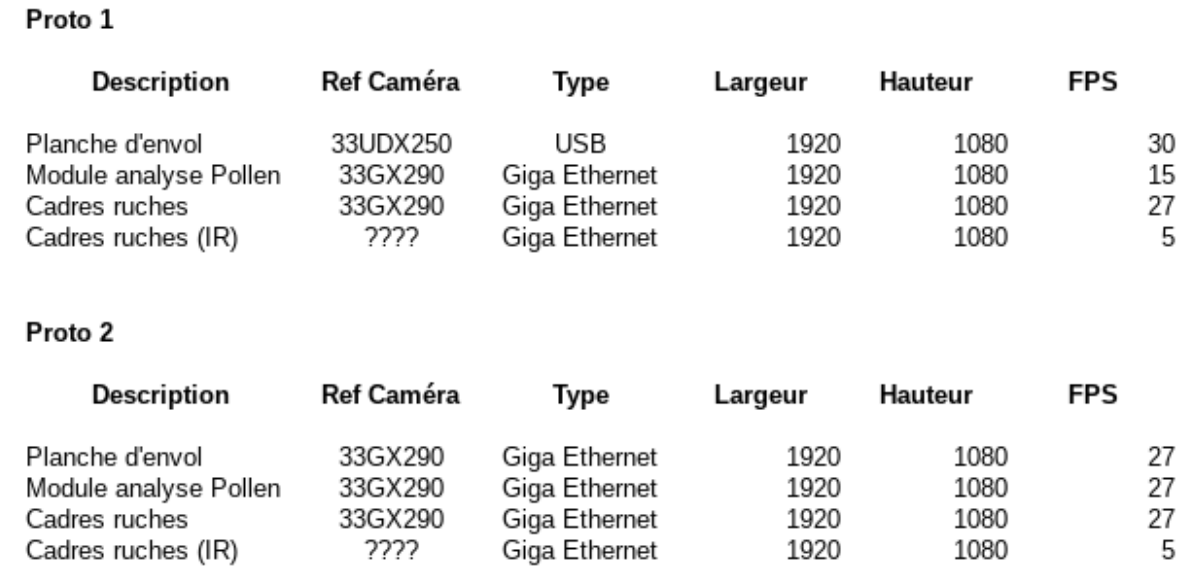
\includegraphics[scale=0.25]{../images/annexes/camera_bp.png} 
    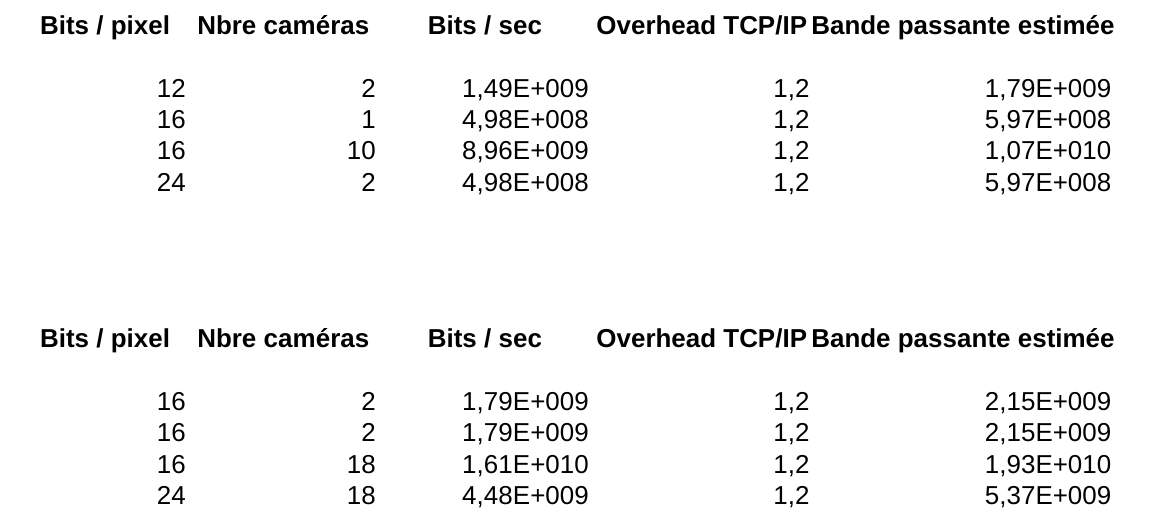
\includegraphics[scale=0.25]{../images/annexes/camera_bp2.png} 
    \caption{Tableau récapitulatif des futures caméras}
    \label{tab_recap_cam}
\end{figure}
Deux prototypes sont présentés, puisque nous comptons accueillir deux prototypes de ruches plates : la nôtre et 
celle qui sera envoyée à nos partenaires allemands ensuite. \\
Les caméras pour la planche d'envol et pour le module d'analyse de pollen seront en couleur. Celles pour les cadres de la ruche
seront monochromes : il avait été prévu des caméras couleurs à la base, mais d'après les biologistes nous en auront pas besoin pour 
repérer ce que nous voulons. Ainsi, nous gagnons en bande passante, les caméras monochromes étant moins gourmandes que les couleurs 
en données. \\
En plus des caméras, il faut prévoir le poids des données des capteurs de la carte électroniques. Ces données sont négligeables par
rapport au reste, mais sont à prévoir. Ces capteurs sont représentés dans le document par une des caméras "Cadres Ruches". 
Enfin, les calculs prévoient également l'en-tête TCP-IP nécessaire à l'envoi des données, cette prévision étant sur évaluée 
pour avoir de la marge. Ainsi, on ajoute 20\% de données supplémentaire.\\
Maintenant, nous savons un peu plus quels seront les données qui transiteront sur notre réseau. Nous avons aussi
quelques contraintes pour le choix du matériel réseau qui sera acheté dès que nous pourrons utiliser le réseau au rucher. \\
Le Switch servira à connecter les caméras, les capteurs, l'ordinateur déjà sur place et notre potentiel matériel supplémentaire
lorsque nous travaillerons sur place. Il devra être un 24 ports POE (Power Over Ethernet) capable 
d'alimenter nos caméras avec la norme SFP + requise par le technicien du CNRS. \\
Le serveur de récolte et de données devra être en double alimentation pour se suppléer l'une et l'autre en cas de panne,
assurant que le serveur tourne encore grâce à la redondance. Il devra avoir un port Ethernet de 20Gb et posséder un CPU multicœur.
Ce serveur doit être commandé chez DELL pour un budget de 15k€ maximum. \\
J'ai déjà fait quelques recherches sur leur site afin d'avoir une idée de ce qui existait, mais la commande étant reportée à cause
du temps d'installation de la fibre au rucher, ces achats sont décalés à plus tard pour le moment.\\ 

        \subsection{Tests pour la vitrine Web}
En plus de l'installation réseau pour la récolte des données, il faudra aussi penser à la façon dont nous allons présenter nos 
résultats. Ce travail servant de présentation, il est moins urgent que la réalisation des captures de données et a été mis de 
côté pendant mon stage. Cependant, j'ai passé une petite journée à me familiariser avec ce type d'installation en faisant 
quelques tests sur un serveur de test prêté par M. Druon. Cette journée a surtout été consacrée à de la documentation en amont,
avec la lecture de quelques tutoriels sur Internet. J'en ai aussi profité pour relire les cours et 
TP du DUT en lien avec les serveurs Webs et le développement Web : base de donnée (M2104), langage HTML/CSS (M1106, M2105)
installation d'apache). 
Pour ce qui est du contenu de cette vitrine Web, je n'ai pas concrètement travaillé dessus mais ai imaginé à quoi celle-ci pourrait
ressembler \footnote{\ref{sch_web}}. \\
\begin{figure}[!h]
    \centering
    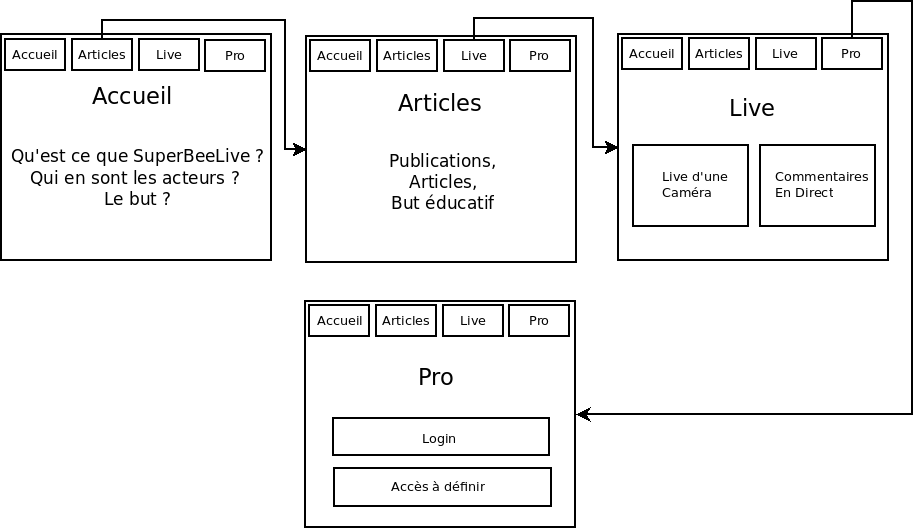
\includegraphics[scale=0.5]{../images/dia/sch_web.png}
    \caption{Proposition de schéma pour la vitrine Web}
    \label{sch_web}
\end{figure}
Ce n'est qu'une proposition qui n'a pas encore été discutée avec le reste de l'équipe mais que je leur fournis. \\
Pour moi, le site pourrait être construit en quatre parties : 
\begin{itemize}
    \item  L'accueil, expliquant ce qu'est notre projet, qui en sont les acteurs
ce qu'on veut en ressortir etc. 
    \item La partie article, contenant des liens vers les publications faites par l'équipe concernant le projet, des articles écrits
spécifiquement pour le site ou des petit compte rendu d'avancement, avec des photos de nos opérations par exemple. Le but 
étant de montrer au public ce qui est fait et de rendre le projet attractif. Il faut que ce soit du contenu simple et rapide
à produire. 
    \item  La partie Live, avec quelques caméras sélectionnées pour le grand public et la description des événements en temps réel par 
        les algorithmes qui seront réalisés par l'équipe. En attendant la réalisation de ces algorithmes, nous pourrions simplement afficher
        le live de quelques caméras sans commentaires. \\
    \item La partie "pro", qui serait un portail de connexion pour les collaborateurs à qui nous voulons partager plus d'informations.
Ils auraient accès à plus de caméras, aux documents techniques, etc. On pourrait y mettre un drive afin de faciliter le partage de 
document. Ce serait une plateforme de travail pour le projet.\\
\end{itemize}
Bien sûr, l'élaboration d'un tel site nécessite des connaissances en web design et en sécurité informatiques. Je me suis penchée
sur la question parce que j'ai trouvé le sujet intéressant et aimerai à l'avenir pouvoir m'y intéresser un peu plus. \\ 

        \subsection{Aide pour les projets de première année à l'IUT de Béziers}
En plus de mon aide sur les travaux cités si dessus, ma présence en tant que stagiaire a aussi été bénéfique pour aider M. Druon 
dans une tâche se détachant un peu du monde de la Recherche : aider durant les projets des étudiants en Réseaux et Télécommunications 
de première année. \\
Ce travail reste en lien avec SuperBeeLive puisque l'IUT de Béziers est partenaire du projet et qu'un des groupe d'étudiants (groupe 13) 
a fait son projet sur la température et l'humidité dans la ruche. \\
C'est pour cela que tous les jeudis je me suis déplacée à l'IUT de Béziers pour être disponible avec M. Druon pour les étudiants de premières
années.
Pendant ces jeudis-ci, je travaillais le matin sur Beeterface et 
l'après midi je continuais de coder en salle projet pour répondre à d'éventuelles questions. \\
J'ai également eu à m'occuper des commandes des étudiants : récolter leur liste de demandes, les regrouper pour faire les commandes
aux fournisseurs, réceptionner, inventorier et ranger \footnote{Voir Figure \ref{photo_bureau}}.\\
\begin{figure}
    \centering
    \includegraphics[scale=0.5]{../images/photos.png}
    \caption{Photo du rangement des commandes}
    \label{photo_bureau}
\end{figure}
    

%TODO Photo du rangement des commandes 
Ma présence sur l'IUT s'est intensifiée pendant les deux semaines où les étudiants étaient à temps plein sur leur projet, du 18 au 30 juin. \\
Durant ces deux semaines, j'ai été affectée au bureau se trouvant à côté du laboratoire de l'IUT où j'avais rangé tous le matériel 
destiné aux projets.
J'ai donc servit de régie, car même après la première distribution du matériel demandé par les étudiants, beaucoup avaient 
besoin de pièce de rechange, de nouvelles pièces, etc. \\
Cela m'a permis de continuer à travailler sur mon code, de manière moins intensive que lorsque je me trouvais au LIRMM, tout en
aidant M. Druon en le déchargeant des demandes de matériel. 
J'ai également aidé à noter les présences et ai fait attention au travail fourni par les étudiants afin de donner un avis extérieur pour
les notations.
Étant souvent dans les couloirs où ils travaillaient, j'ai aussi répondu à beaucoup de questions et demandes d'aide : 
j'essayai de répondre au mieux, de les diriger pour qu'ils trouvent la réponse d'eux même ou de les envoyer voir M. Druon si 
j'estimais que la question nécessitait un œil plus expert. \\
Au moment des soutenances, j'ai participé à un Jury devant normalement se tenir avec deux professeurs, mais M. Druon se retrouvant 
finalement seul dans celui-ci par manque d'effectif, c'est en binôme que nous avons écouté le travail des étudiants.
D'autres deuxièmes années ou redoublant se trouvaient dans les trois autres jurys avec d'autres professeurs. 
L'exercice de notation a été un peu difficile : bien qu'ayant un peu peur de noter injustement,
je savais très bien que la note qui allait être la plus importante serait celle 
du professeur. Néanmoins, c'était très intéressant de se retrouver de l'autre côté et d'évaluer des travaux que, moi-même, 
j'avais dû effectuer il y a un an. \\
Ces missions annexes m'auront permis d'appliquer concrètement plusieurs notions vues pendant le DUT. \\
Théorique d'abord, avec les calculs pour la bande passant nécessaire pour le rucher et le questionnement sur le matériel à commander, ainsi
qu'avec les recherches autour du développement et l'installation web. 
J'ai aussi pu revoir beaucoup de sujets pratiques avec les étudiants de première année : beaucoup de leur question tournaient autour 
de choses que j'avais déjà fait, en cours ou en projet,  mais sur lesquels il me manquait expériences et connaissances à ces moments-là et
qui ne me posent plus problème aujourd'hui. \\

    \section{Compétences développées} \\
Lors de stage de fin d'études, j'ai pu appliquer beaucoup de connaissances que j'ai acquises pendant ces deux dernières années,
mais aussi apprendre beaucoup à différents niveaux.\\
Mon rôle principal dans l'équipe n'étant pas de faire de l'administration réseaux et systèmes tous les jours, 
j'ai pu utiliser mes connaissances dans ce domaine d'une autre manière qu'en administrant des infrastructures déjà installées. \\ 
C'est surtout la théorie qui m'aura été utile, voyant plus le rôle d'un ingénieur que d'un technicien. 
Mes journées de travail se passant en grande majorité sur un ordinateur, j'ai au quotidien fait de l'administration Unix et ai
utilisé des outils que je ne connaissais que partiellement avant. Ainsi, mon but était d'être plus rapide avec ces outils 
et j'ai donc appris des raccourcis clavier et des techniques que me conseillaient les personnes autour de moi pour optimiser 
mon temps. \\
De plus, j'ai ensuite eu la chance d'avoir un ordinateur fourni par le LIRMM, également sous Unix.
Comme cette machine m'était destinée, j'ai pu passer du temps à la configurer comme je le voulais : 
installation d'une interface graphique (i3), configuration de VIM \footnote{Voir bibliographie \cite{ref6}}, d'un terminal personnalisé, personnalisation des couleurs 
sur mon shell, test d'une alternative à bash (fish) etc. 
Si je considère cette partie personnalisation, comme une compétence développée pendant le stage, c'est parce que j'ai eu la chance 
d'avoir autour de moi une équipe pour qui il était important que je sois à l'aise avec mes outils de travails, me laissant une 
journée pour travailler là-dessus. \\
Je pense ainsi avoir aujourd'hui bien plus d'aisance derrière une machine sous Unix qu'il y a 3 mois. \\
J'ai aussi beaucoup appris pendant les deux semaines d'encadrement d'étudiant. Même si je n'avais pas le statut de professeur 
ou de vacataire, ma place en tant que "seconde" de M. Druon auprès des premières années était bien ancrée 
et m'a permis de voir le nombre de compétences nécessaire pour faire un tel travail : patience, organisation, 
capacité à expliquer les concepts et endurance s'ajoutent aux connaissances nécessaire pour aider des étudiants. 
Enfin, les compétences que j'ai les plus développées sont bien entendu celles autour de la programmation. 
À mon arrivée dans l'équipe, je ne pensais pas que j'allais autant me consacrer au code : je n'étais pas très à l'aise avec ça 
pendant mes deux années de DUT et avais un peu peur de me lancer dans des projets d'envergures dans ce domaine. 
Mais une fois sur place et lancée, j'ai appris énormément en peu de temps. Je pense même pouvoir dire que j'ai rattrapé le retard 
que j'avais pris lors de mon DUT avec ces trois mois presque intensif sur le sujet. \\
J'ai bien mieux compris comment utiliser les outils de compilations et comment cette étape se déroulait. L'algorithmie m'est bien moins
effrayante, le langage C est devenu pour moi une référence et je continue d'en apprendre dessus régulièrement. 
Il ne me reste d'ailleurs plus qu'un pas avant d'attaquer le langage objet grâce à GTK : cette partie de la programmation très graphique
me plaît énormément et c'est ce qui, je pense, m'a réconciliée avec la programmation. \\
Désormais, je travaille beaucoup avec GIT sur GitHub, en découvrant des projets disponibles dessus et en partageant mes scripts,
mes configurations Unix, etc. 
En soit, j'aurai appris sur beaucoup de sujets différent, plus que ce que je n'aurai pu l'imaginer.
J'ajoute aussi qu'au moment où j'écris ces lignes, j'apprends à me servir de Latex, un langage de composition de document, 
puisque je rédige mon rapport de stage avec cet outil \footnote{Voir bibliographie \cite{ref4} \cite{ref9}}.\\

Pour conclure, ce stage au sein de l'équipe SuperBeeLive m'aura apporté un bon nombre de choses : des compétences, des connaissances, mais 
aussi de l'aisance. C'est avec les mises en application de mes connaissances acquises lors du DUT que j'ai pu prendre confiance en celle-ci.
De plus, j'ai acquis un bon nombre de nouvelles connaissances, aussi bien concernant le monde biologique qui entoure les abeilles que sur 
divers sujets se rapprochant de l'informatiques aux systèmes embarqués. Ces connaissances s'étendent la culture générale à des applications 
concrètes.\\
Ainsi, ces trois mois m'auront permis d'apprendre à travailler différemment que dans un milieu scolaire. 


\chapter{Conclusion}
Ces trois mois de stages auront été formateurs pour moi sur plein d'aspects. Ayant déjà connaissance du travail en entreprise depuis un an
avec un boulot d'été que j'avais eu dans une entreprise de développement logiciel, j'ai pu découvrir un autre milieu de travail : 
la recherche. \\
Dans ce cadre, notre équipe de projet était moins souvent réunies, vu que ce sont plusieurs laboratoires qui travaillent ensemble, 
mais elle n'en reste pas moins soudée et très agréable. Les trois personnes avec qui j'ai le plus eu de contact, Sébastien Druon, 
Capucine Carlier et Matthieu Rousset étaient tous trois présents à leur niveau pendant mon stage.  \\
Bien que j'avais connaissance de ce que j'allais faire globalement dans l'équipe, j'ai été surprise lorsque j'ai su que j'allais
devoir concevoir une application et surtout devoir m'occuper entièrement de l'interface de celle-ci. 
Ayant des difficultés en programmation à mon arrivée dans l'équipe, ce travail me paraissait bien plus difficile que ce qu'il 
en a été réellement. Le fait qu'on me laisse du temps pour que je puisse me former convenablement sur le sujet m'aura été 
d'une grande aide. Par ailleurs, n'ayant pas de mal à apprendre en autodidacte, j'ai beaucoup travaillé avec des livres et
des sites internet, tous retrouvables dans la bibliographie. En plus de ces ressources, M. Druon a pris beaucoup de temps
pour répondre à mes questions et m'aider à des endroits où je bloquais, peu importe le domaine. \\

Ma participation lors des projets des premières années aura été pour moi une expérience nouvelle et très enrichissante. Voir
d'autres étudiants à la place que j'avais il y a un an m'a fait prendre conscience du chemin parcouru lors de mes deux années de DUT. 
Venant d'un Bac Littéraire, ces deux années dans un milieu plus scientifiques n'auront pas été de tout repos. Malgré les difficultés, 
j'ai pu terminer mon DUT sur un stage très intéressant et épanouissant.
C'est d'ailleurs avec une grande joie que je rejoins l'équipe de SuperBeeLive pour encore trois ans. Ma candidature pour l'école d'ingénieurs
à Polytech section Systèmes Embarqués en apprentissage ayant été acceptée, j'ai signé mon apprentissage au LIRMM. \\
Je vais donc encore pouvoir suivre l'évolution du projet et finir ce que j'ai commencé, que ça soit l'application, la mise en place du 
réseau et pouvoir commencer la vitrine web et les cartes électroniques.  \\

\bibliographystyle{plain}
\bibliography{biblio}

\chapter{Annexes}
\begin{figure}[t]
    \centering
    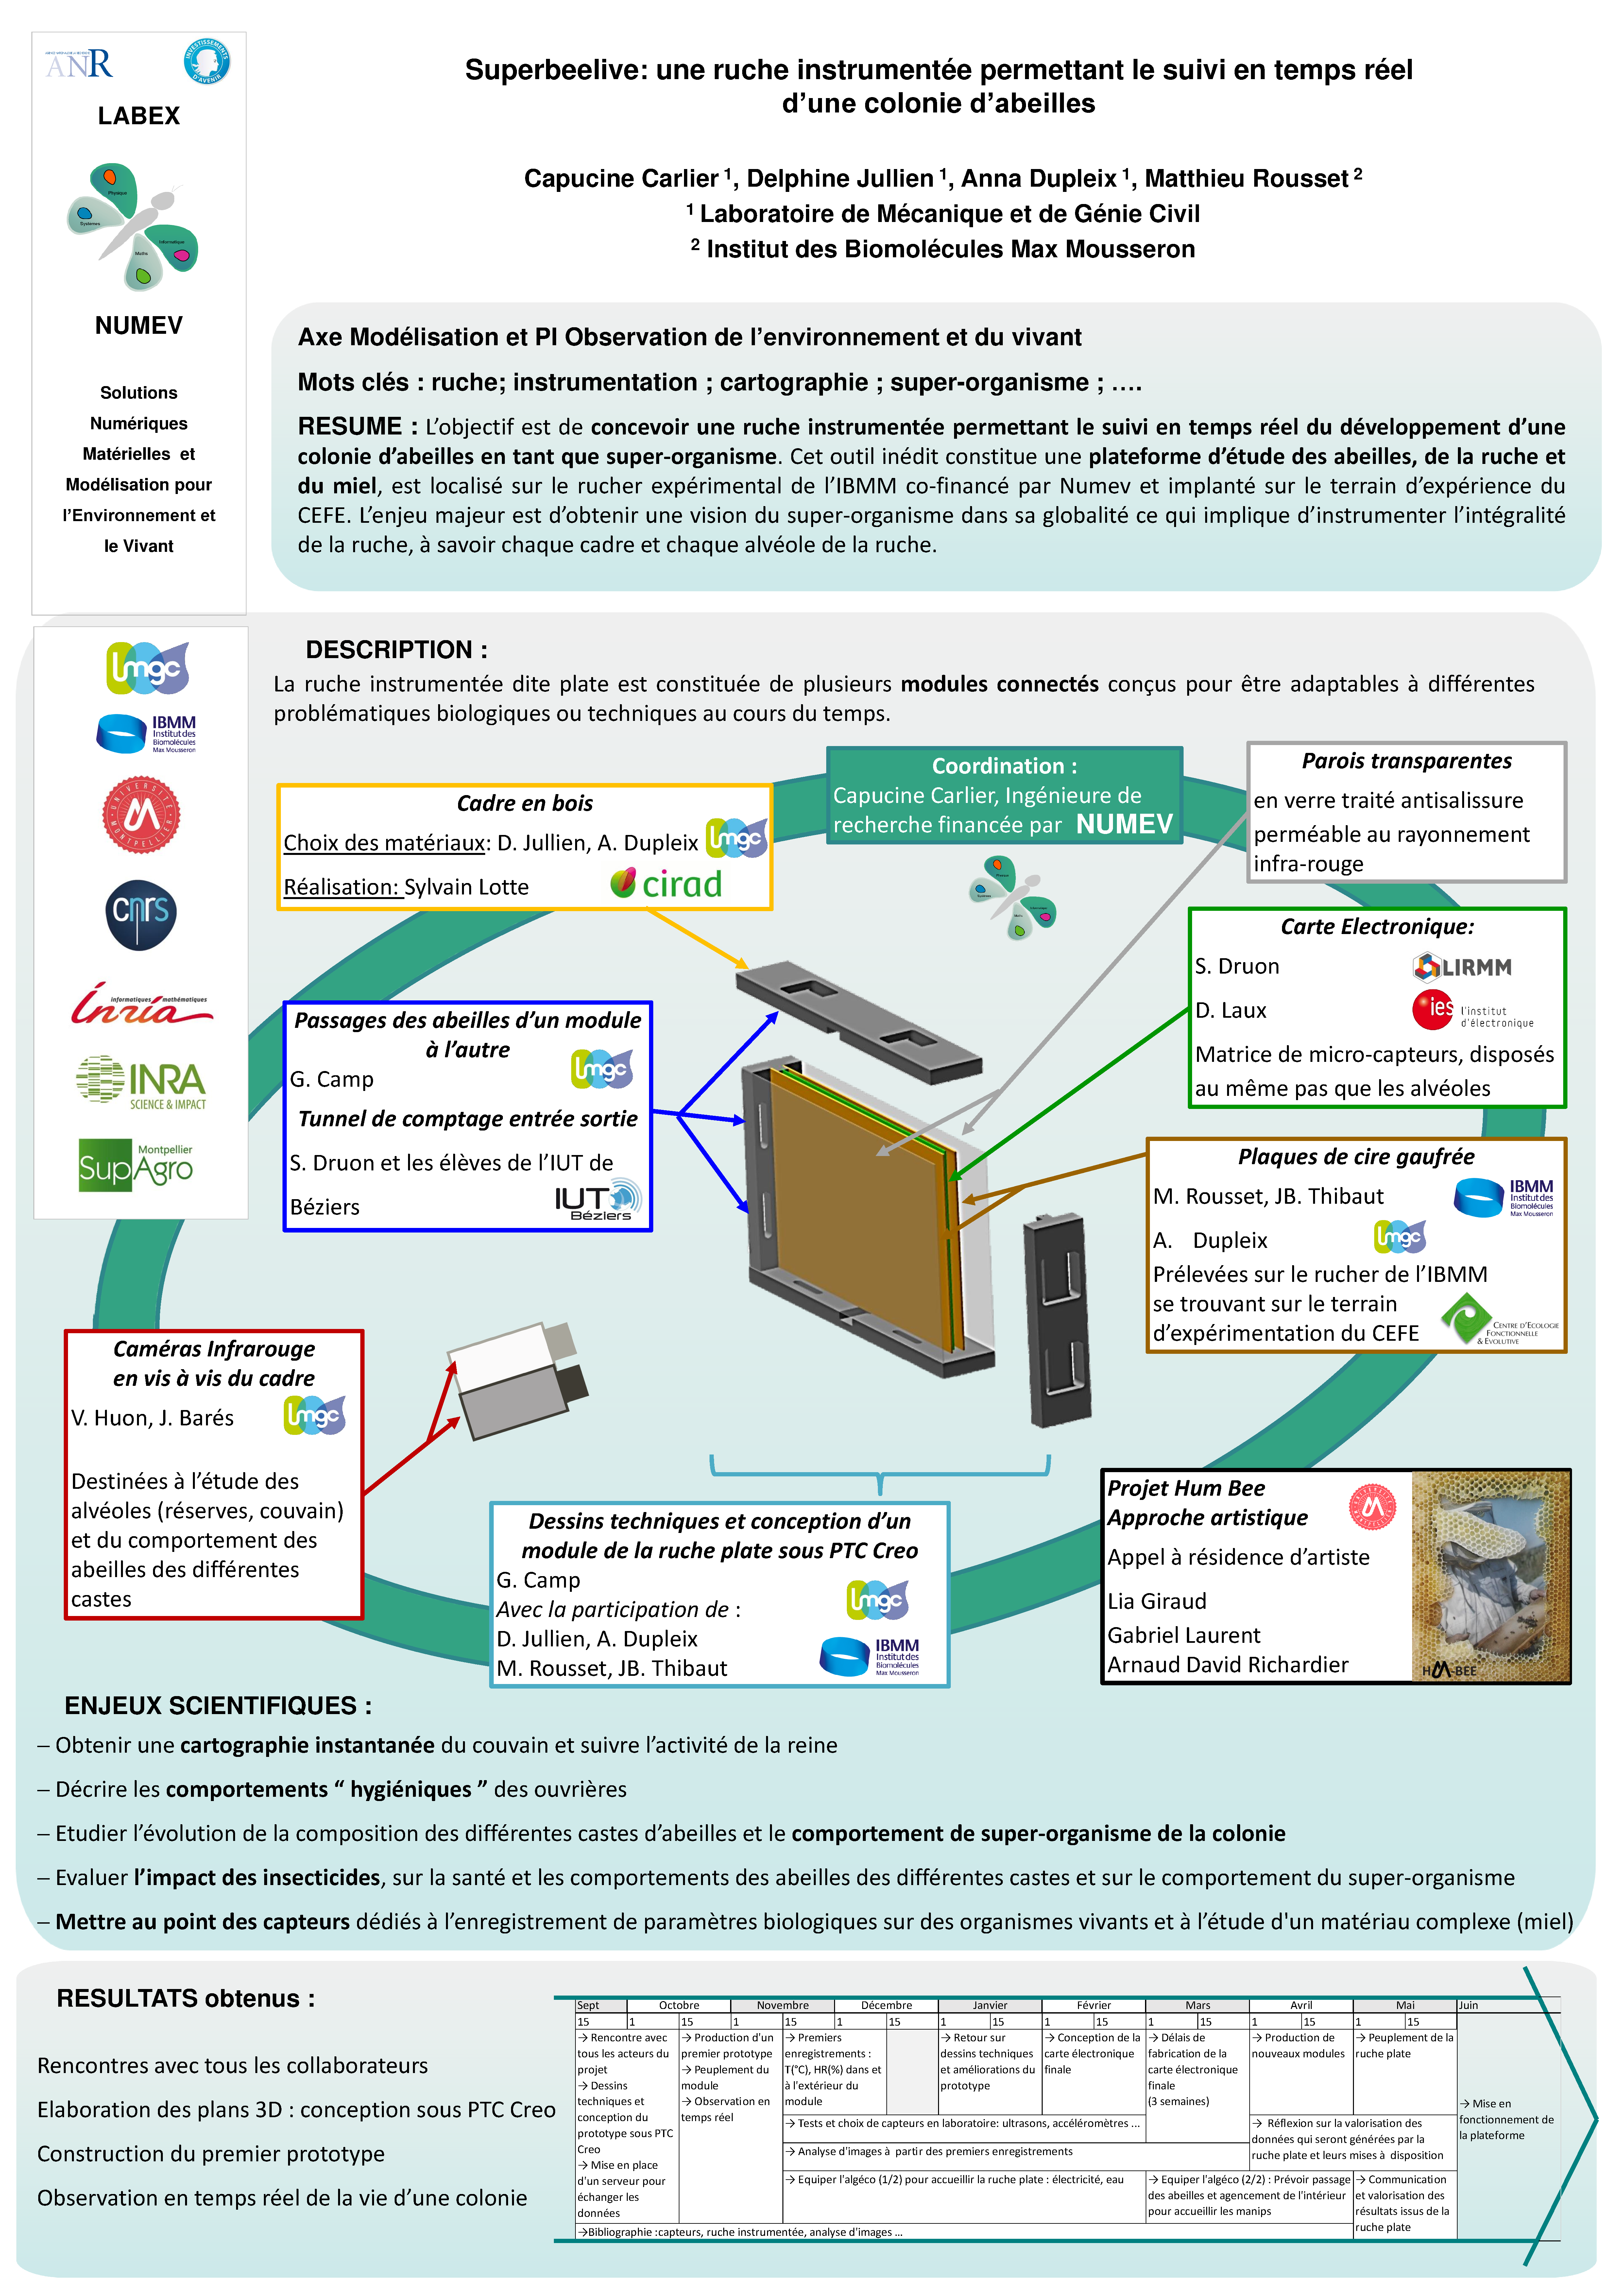
\includegraphics[scale=0.2]{../images/annexes/poster_numev.pdf}
    \caption{Poster NUMEV}
    \label{an1}
\end{figure}

\begin{landscape}
    \begin{figure}[h]
    \centering
    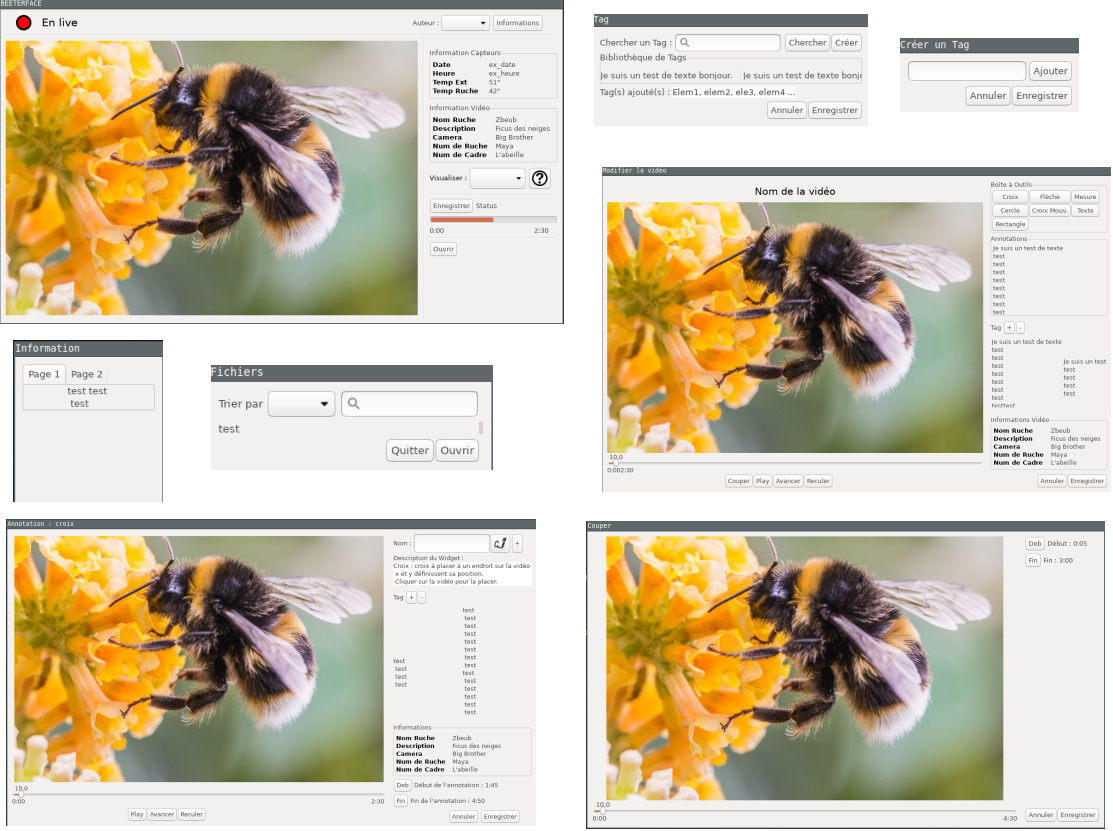
\includegraphics[scale=0.6]{../images/annexes/screen_appli.png}
    \caption{Screenshots de l'application Beeterface}
    \label{an2}
\end{figure}
\begin{figure}[h]
    \centering
    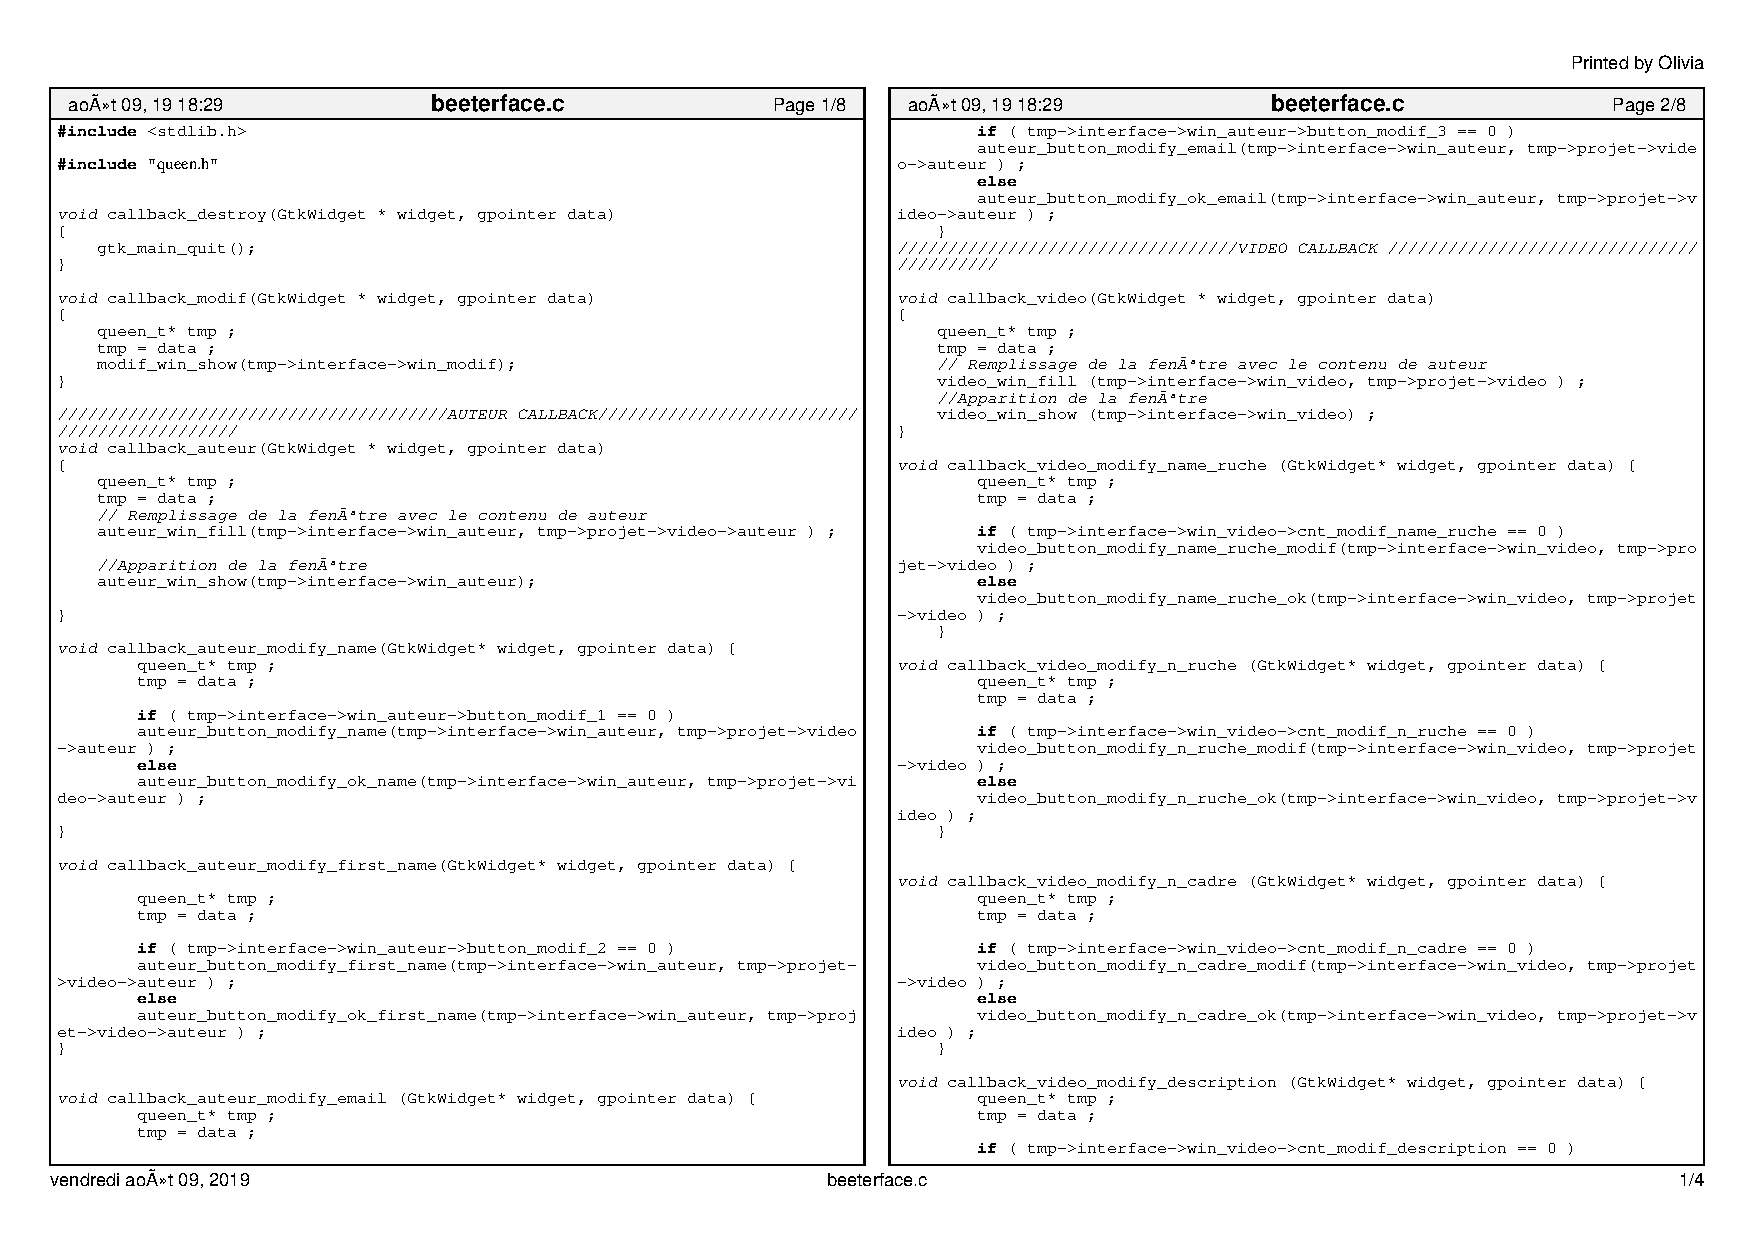
\includegraphics[page=1,scale=0.8]{../code/beeterface.pdf}
    \caption{beeterface.c}
    \label{an3}
\end{figure}

\begin{figure}[h]
    \centering
    \includegraphics[page=2,scale=0.9]{../code/beeterface.pdf}
\end{figure}

\begin{figure}[h]
    \centering
    \includegraphics[page=3,scale=0.9]{../code/beeterface.pdf}
\end{figure}

\begin{figure}[h]
    \centering
    \includegraphics[page=4,scale=0.9]{../code/beeterface.pdf}
\end{figure}
\end{landscape}


\begin{landscape}
\begin{figure}[h]
    \centering
    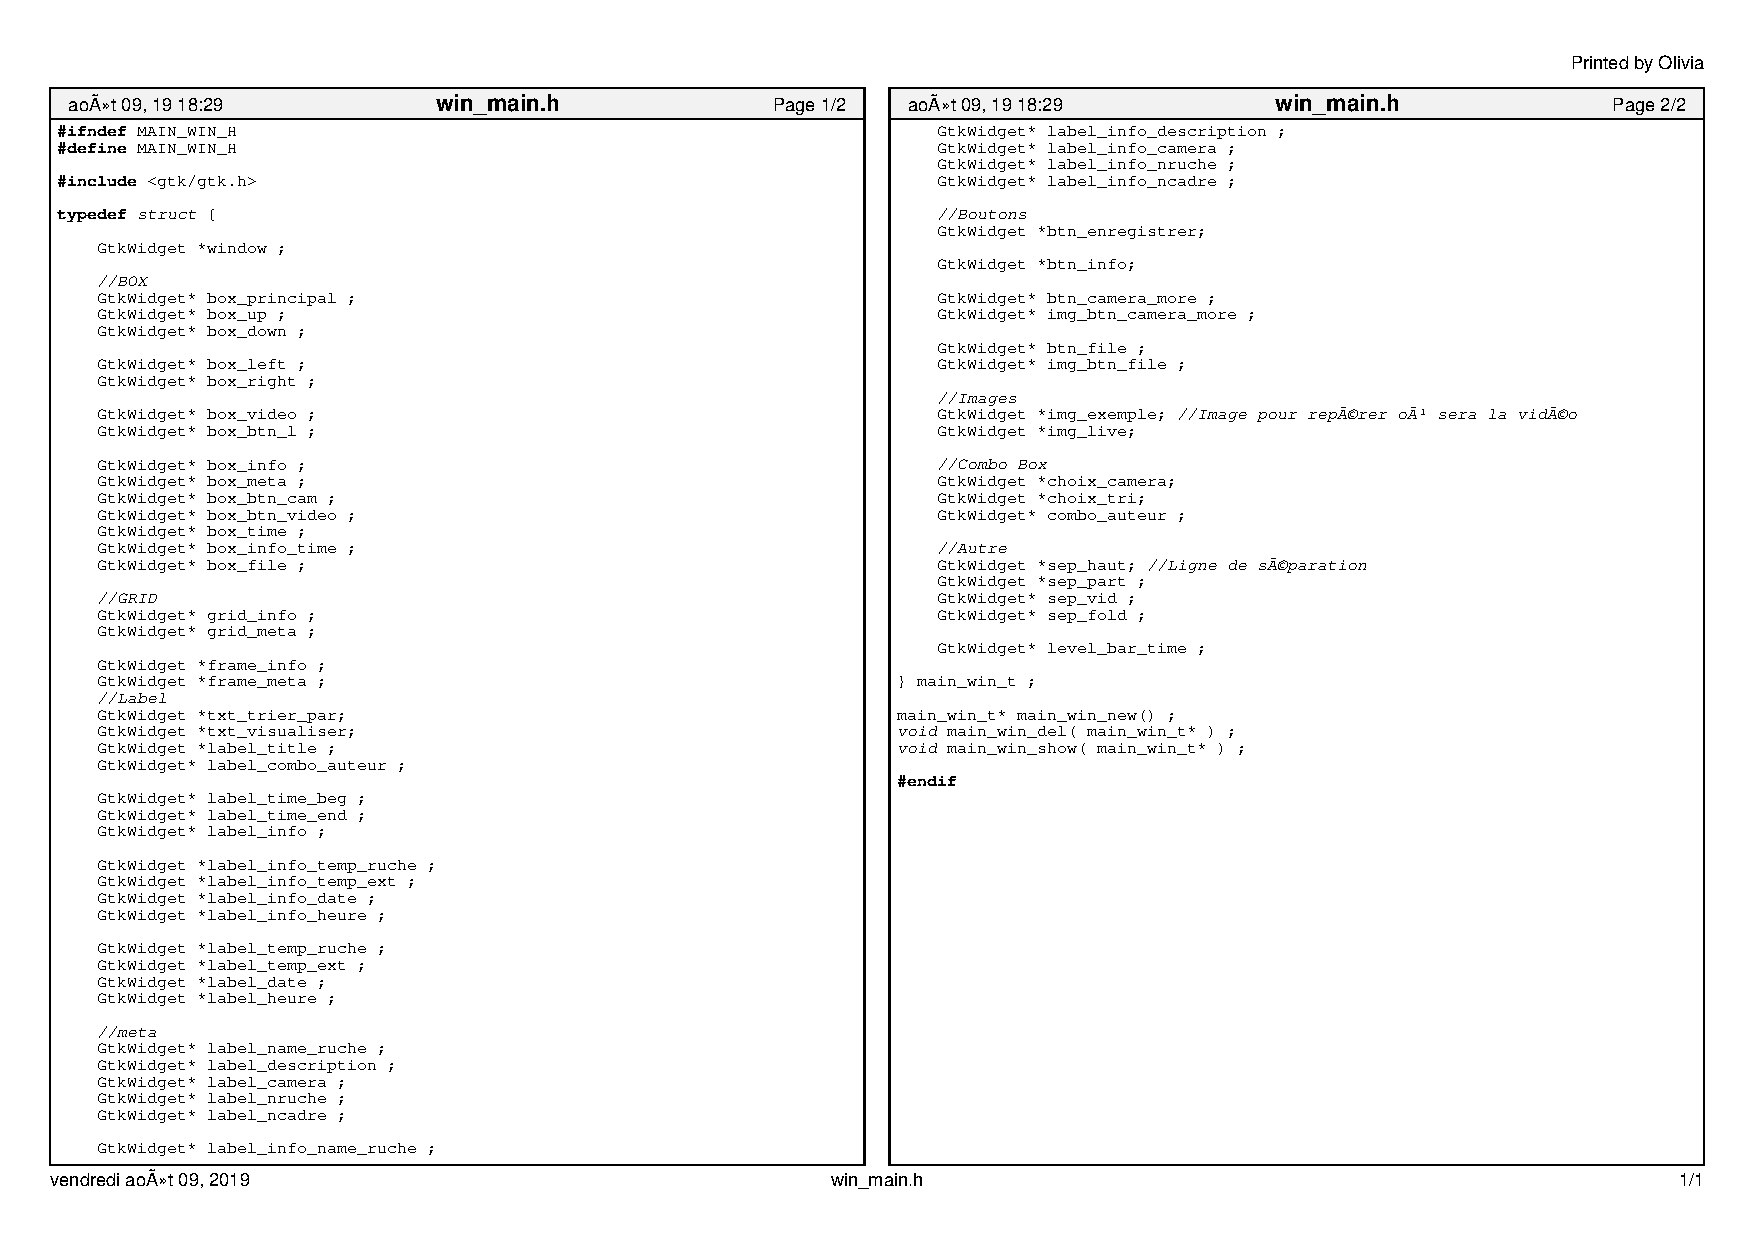
\includegraphics[page=1,scale=0.85]{../code/win_main_h.pdf}
    \caption{win\_main.h}
    \label{an4}
\end{figure}
\end{landscape}

\begin{landscape}
\begin{figure}[h]
    \centering
    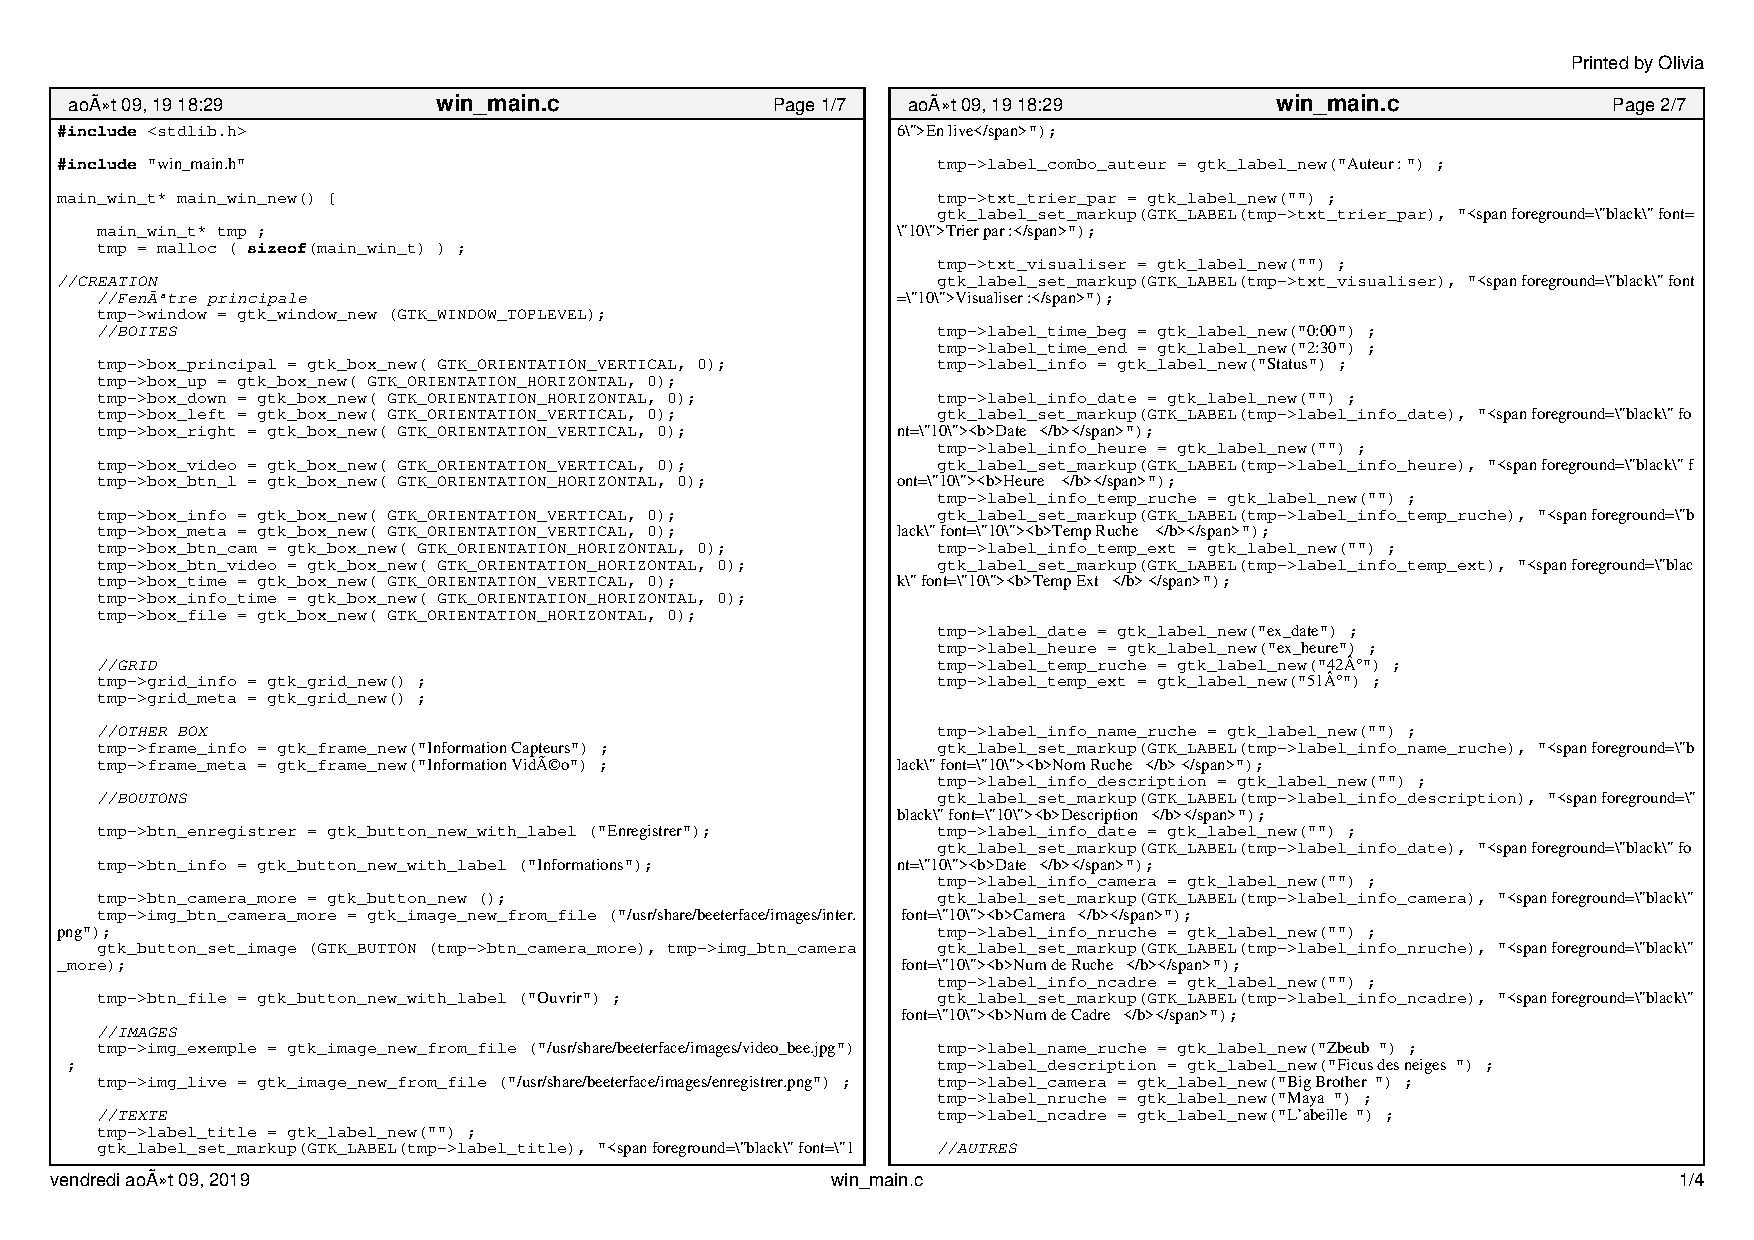
\includegraphics[page=1,scale=0.85]{../code/win_main_c.pdf}
    \caption{win\_main.c}
    \label{an5}
\end{figure}
\end{landscape}

\begin{landscape}
\begin{figure}[h]
    \centering
    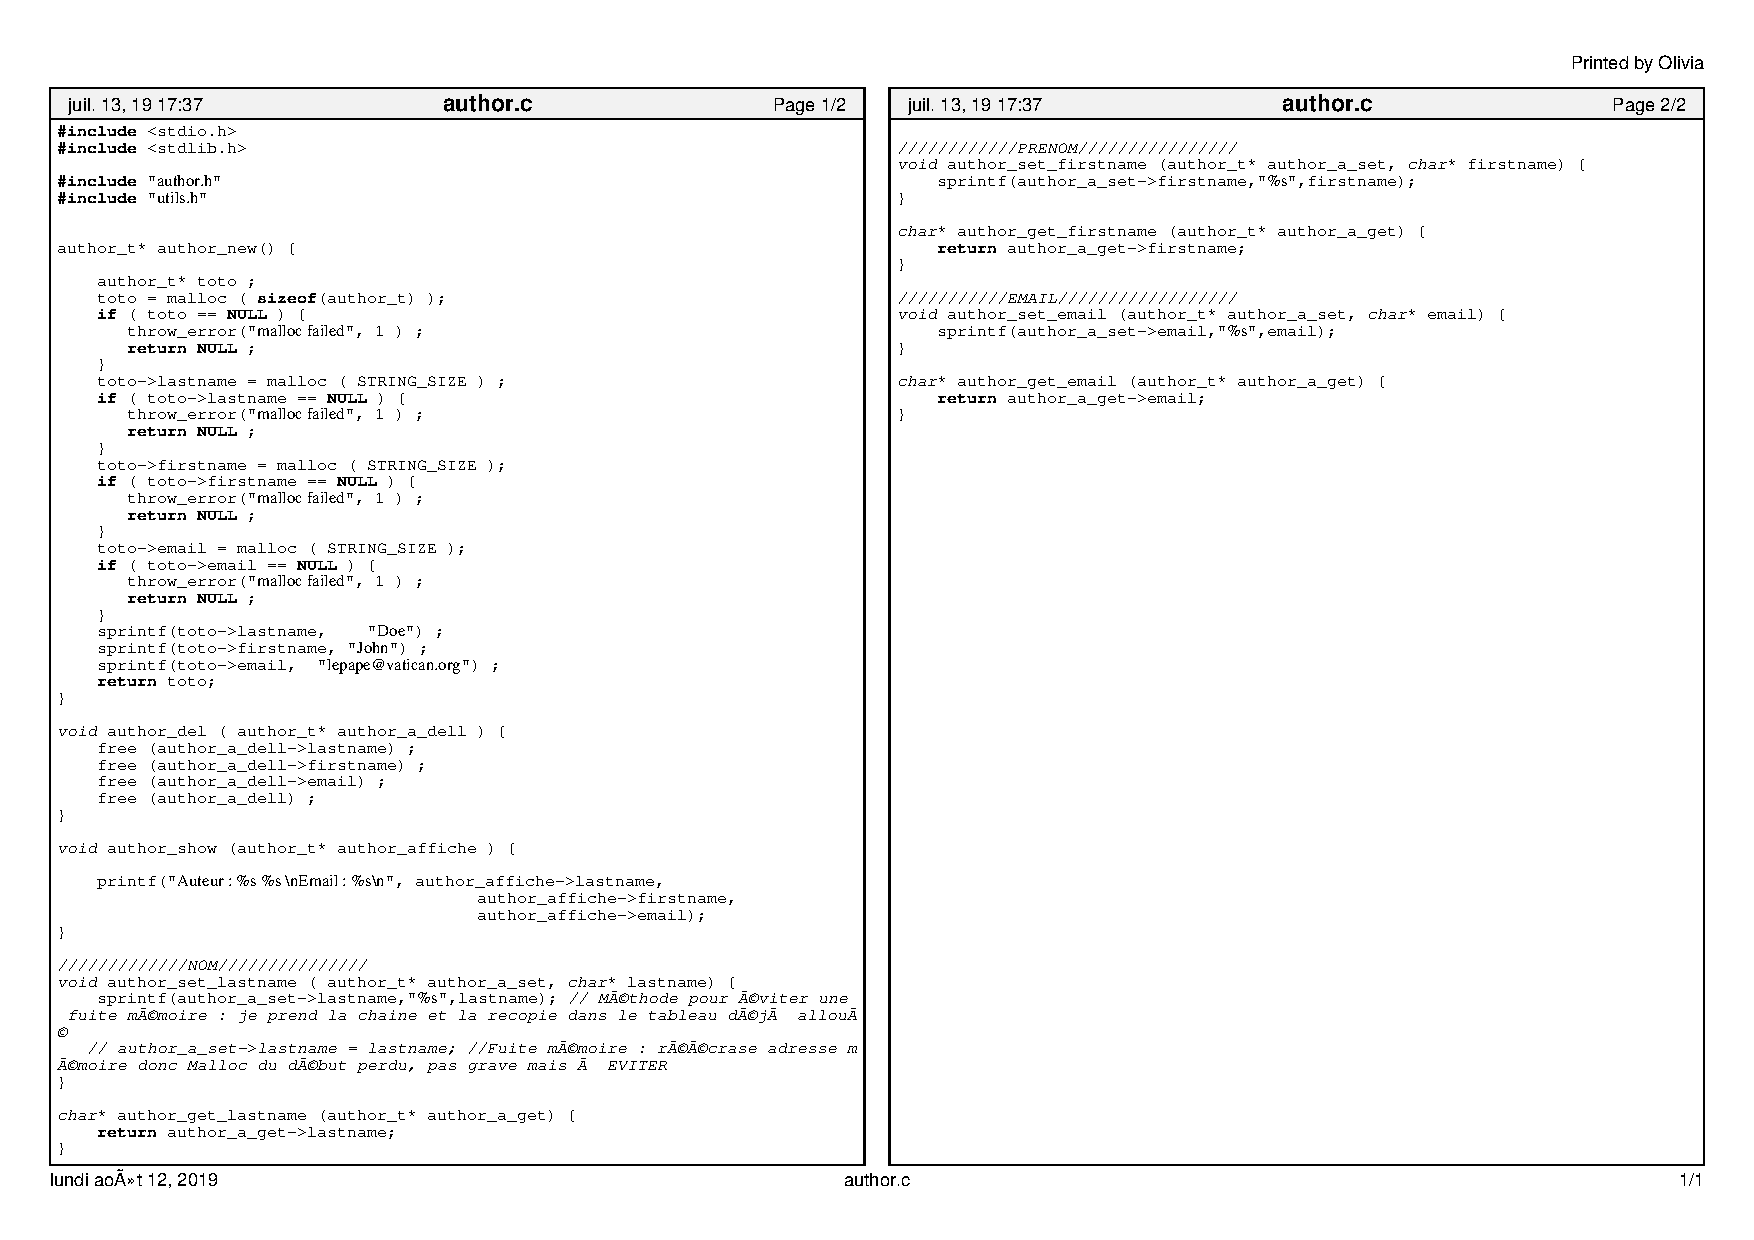
\includegraphics[page=1,scale=0.85]{../code/author.pdf}
    \caption{win\_main.c}
    \label{an6}
\end{figure}
\end{landscape}
\end{document}







